 \newpage
 \vskip 6mm
 \pagestyle{myheadings}
 \markboth{{\underline{\centerline{东南大学博士学位论文} }}}
 {{\underline{\centerline{第四章 \ \ \  基于多级小波分解和传递熵的车辙预测建模和影响因素分析混合框架} }}}
 
 \chapter{基于多级小波分解和传递熵的车辙预测建模和影响因素分析混合框架}\label{ch4}
 \setcounter{equation}{0}
\section{引言}
在前两章中,我们对以传递熵为基础的因果关系模型进行了理论和方法上的创新。从本章开始,我们将展示基于传递熵的因果网络在复杂系统中建模的应用。以沥青路面车辙预测模型为例,本章将展示因果网络作为模型中特征选取模块的应用。
车辙作为沥青路面的一种主要破坏形式,不仅会导致路面结构性能衰减,还会加速路面损坏。此外,车辙还会威胁行车安全,对正常交通极为不利\cite{1,2}。同时,由于车辙变形既发生在沥青路面的面层,也发生在下层,因此车辙的养护工作十分困难\cite{3}。车辙问题的解决不仅有赖于抗车辙材料的研发和沥青路面抗车辙性能的提高,还可以在设计阶段根据路面的影响因素预测车辙变形的发展,从源头上保证路面的抗车辙性能\cite{4}。因此,高精度车辙预测模型的研究对于评价车辙病害、提高路面使用寿命具有重要意义。
近年来,车辙预测研究取得了长足的发展。然而,以下两个突出问题依然存在,并严重制约了车辙预测性能及其应用。第一个问题是缺乏有效的、通用的数据处理、特征选择和建模框架。车辙预测模型的研究需要分析车辙变形的影响因素,车辙变形是沥青路面在交通荷载因素、气候环境因素和路面材料因素的耦合作用下产生的永久变形。常见的经验模型是基于多元回归分析,这种方法会忽略历史数据的依赖性。因此,时间序列模型通常用于研究复杂系统并了解其随时间变化的行为方式(cite{5})。从统计学角度来看,时间序列模型的一般定义可表述为:
\begin{eqnarray}
\hat{y}_{i,t+n} = f(Y_{i,t-k},X_{j,t-k},s), \nonumber
\end{eqnarray}
其中,模型输出 $\hat{y}_{i,t+n}$ 为序列,$n$ 为预测步数;$Y_{t-k}=\{y_{t},y_{t-1},...,y_{t-k}\}$ 是 $\hat{y}$ 的历史数据;$i$ 是前提条件维度,在本任务中等于 1;$X_{j,t-k}=\{x_{j,t},x_{j,t-1},...,x_{j,t-k}\}$是输入变量序列,$j$代表输入维度;$s$是与实体相关的静态信息。上述三项构成了模型的整个输入,而 $f: R^{i\times k}\rightarrow R^{m}$是待确定的预测模型。随着统计学和大数据的发展,基于机器学习和深度学习的车辙预测模型已被引入,有助于实现长期时间序列建模\cite{6}。特别地,作为复杂系统数据处理的常用技术,时间序列分解通常用于识别原始时间序列的趋势分量和波动分量\cite{7}。此外,基于因果关系的特征值对于建立可解释且稳健的预测模型也有潜在的益处 \cite{5}。


第二个问题是缺乏可信的沥青路面数据。沥青路面的数据来源主要包括:实验室试验、加速路面试验(APT)、路面长期性能跟踪(LTPP)等。与实验室试验和 LTPP 研究相比,加速路面试验不仅能更真实地反映路面的使用状态,而且能在更短的时间内获得路面的使用状态数据。因此,全尺寸轨迹作为一种收集多种路面结构和材料时空性能数据的典型 APT 方法,已被许多国家的研究机构和研究人员广泛采用。交通运输部公路科学研究院轨道(RIOHTrack)是我国第一条全尺寸轨道,于2017年在北京建成\cite{9}。
为克服上述问题,本文提出了一种基于小波分解和多元转移熵的新型车辙预测框架,旨在以可解释的分析方法捕捉车辙及其影响因素之间的因果关系,准确预测车辙演变曲线。本文提出的框架包括三个模块:基于多级离散小波分解(MDWD)的数据处理模块、基于多元传递熵(MTE)的特征选择模块和基于机器学习模型的预测模块。在车辙预测模块中,使用了两个预测模型进行车辙预测,分别是用于预测高频分量的多元高斯过程回归模型(GPR)和用于预测低频分量的双向门控循环单元(bi-GRU),并进一步提供了基于这两个模块的一些因果关系分析。最后,预测结果通过反小波变换进行重构,将各频段的预测结果融合为框架的输出结果。性能比较结果表明,所提出的框架比一些最先进的基线时间序列预测模型更有效。此外,本章还设置了消融实验,以评估每个模块对框架性能的影响。

\section{相关工作}
\subsection{车辙预测模型}
沥青路面车辙评价机理可分为三个阶段\cite{10}。第一阶段是初始沥青混合料的压实过程。该阶段的车辙是人工为提高路面承载能力而产生的。第二阶段为稳定阶段,车辙是沥青混合料在高温或重载作用下抗剪能力不足而产生的流动变形。两侧的隆起量逐渐与凹陷量相等。这一阶段车辙演变的速度相对较慢。第三阶段为快速发展阶段,沥青混合料骨架结构的重新排列过程和沥青混合料的剪切破坏是车辙产生的主要原因。在这一阶段,车辙加深的速度明显加快。从以上分析可以看出,沥青路面车辙主要是沥青层在外部环境因素和内部结构因素的双重作用下产生的流动变形\cite{11,12}。
近年来,人们在车辙预测模型方面做了大量工作。车辙预测模型可分为三类:力学模型、经验模型和力学-经验模型。力学模型以弹性或粘弹性-塑性分层体系理论为基础,通过分析材料变形与应力、应变之间的关系来预测沥青路面的车辙深度。\cite{13}根据实验室蠕变试验的结果提出了修正的麦克斯韦模型。\cite{14}提出了带有时间和温度因子的臼化 Burgers 模型。cite{15}利用统计学原理分析了车辙与其他影响因素之间的关系,并在此基础上建立了预测车辙的经验模型。\cite{16}提出了车辙预测模型,并分析了多变量影响因素。引入了一些深度学习模型以提高车辙预测模型的准确性。\cite{17}提出了基于多层感知(MLP)的车辙演变模型。力学-经验模型基于力学理论建立车辙预测模型,并通过实词数据计算参数。其代表作是 AASTO2002 模型,该模型提供了一种称为 MEPDG 的模型设计方法,用于建立各层的车辙预测模型。M-E模型的参数训练可以采用多元线性回归(MLR)和随机预测的方法,这样可以提高50\%的精度\cite{19}。

\subsection{路面材料和结构的非稳态时间序列预测}
实践中的复杂系统往往表现出多变量非稳态演化行为,所获得的系统信息通常是不完整和不确定的。一般来说,对于沥青路面车辙演变预测这样的典型复杂任务,很难建立精确的分析数学模型。因此,通常通过观测或实验获取时间序列来分析复杂系统。非平稳时间序列预测旨在分析多变量之间的关系,了解纵向观测数据的依赖性,历来是学术界研究的热门领域,应用广泛。从广义上讲,非平稳时间序列的预测模型可分为参数模型和非参数模型,这取决于模型是采取预定义的形式还是纯粹由数据驱动的构造\cite{20}。

参数预测模型通常提供一个具有有限数量参数 $\theta$ 的显式函数来描述输入 $X$ 和输出 $Y$ 之间的关系,其中 $\theta$ 是通过时间序列变现来优化的\cite{21}。作为静态时间序列的经典自回归模型,ARIMA 通过差分来降低非静态性。\cite{22}使用基于 ARMIA 的模型,通过建立结构时间序列来预测交通基础设施。基于神经网络和深度学习的方法因其强大的拟合能力和无需静态假设而被广泛应用于非静态时间序列预测任务中。本文提出了一种基于特征融合 LSTM-BPNN 的路面性能预测模型,并引入了注意力机制 \cite{23}。基于支持向量机(SVM)的模型是另一种经典的参数模型,例如,\cite{24}提出了一种基于粒子群优化(particle swarm optimization,PSO)和支持向量回归(support vector regression,SVR)的沥青路面性能预测模型。

与参数模型相比,非参数模型是在大量观测数据的基础上表示非平稳的动态变化,不需要结构假设和复杂的建模。\cite{20}和\ cite{25}在路面裂缝问题上测试并比较了多种非参数机器学习方法,包括随机森林、朴素贝叶斯和 K-近邻算法。\cite{26} 将经验模态分解(empirical mode decomposition,EMD)引入路面裂缝分析。\cite{27}使用小波分解处理车辙深度时间序列数据,并用ARIMA预测车辙,该方法可以捕捉时间序列的频率特性进行车辙预测。

  
\section{模型描述}
本章提出的多元时间序列分析方法可分为三个模块:(1)基于多级小波分解(MDWD)的数据处理;(2)基于多元传递熵(MTE)的因果推断;(3)混合时间序列预测模型。该方法的架构如图\ref{fig4_1} 所示,其中 MDWD 模块和 MTE 模块在框架的多尺度因果特征检测中发挥了重要作用。基于 MDWD 模块,原始时间序列被分解为低频分量和高频分量,分别代表原始时间序列的趋势项和波动项。然后,MTE 模块选择与车辙具有显著静态偶然关系的影响因素作为各频段时间序列预测模型的特征。最后,对各频段的预测序列进行重构,设计基于融合注意力机制的预测模型,生成车辙预测结果。本节接下来将详细介绍这三个模块。

\begin{figure*}[ht]
\begin{center}
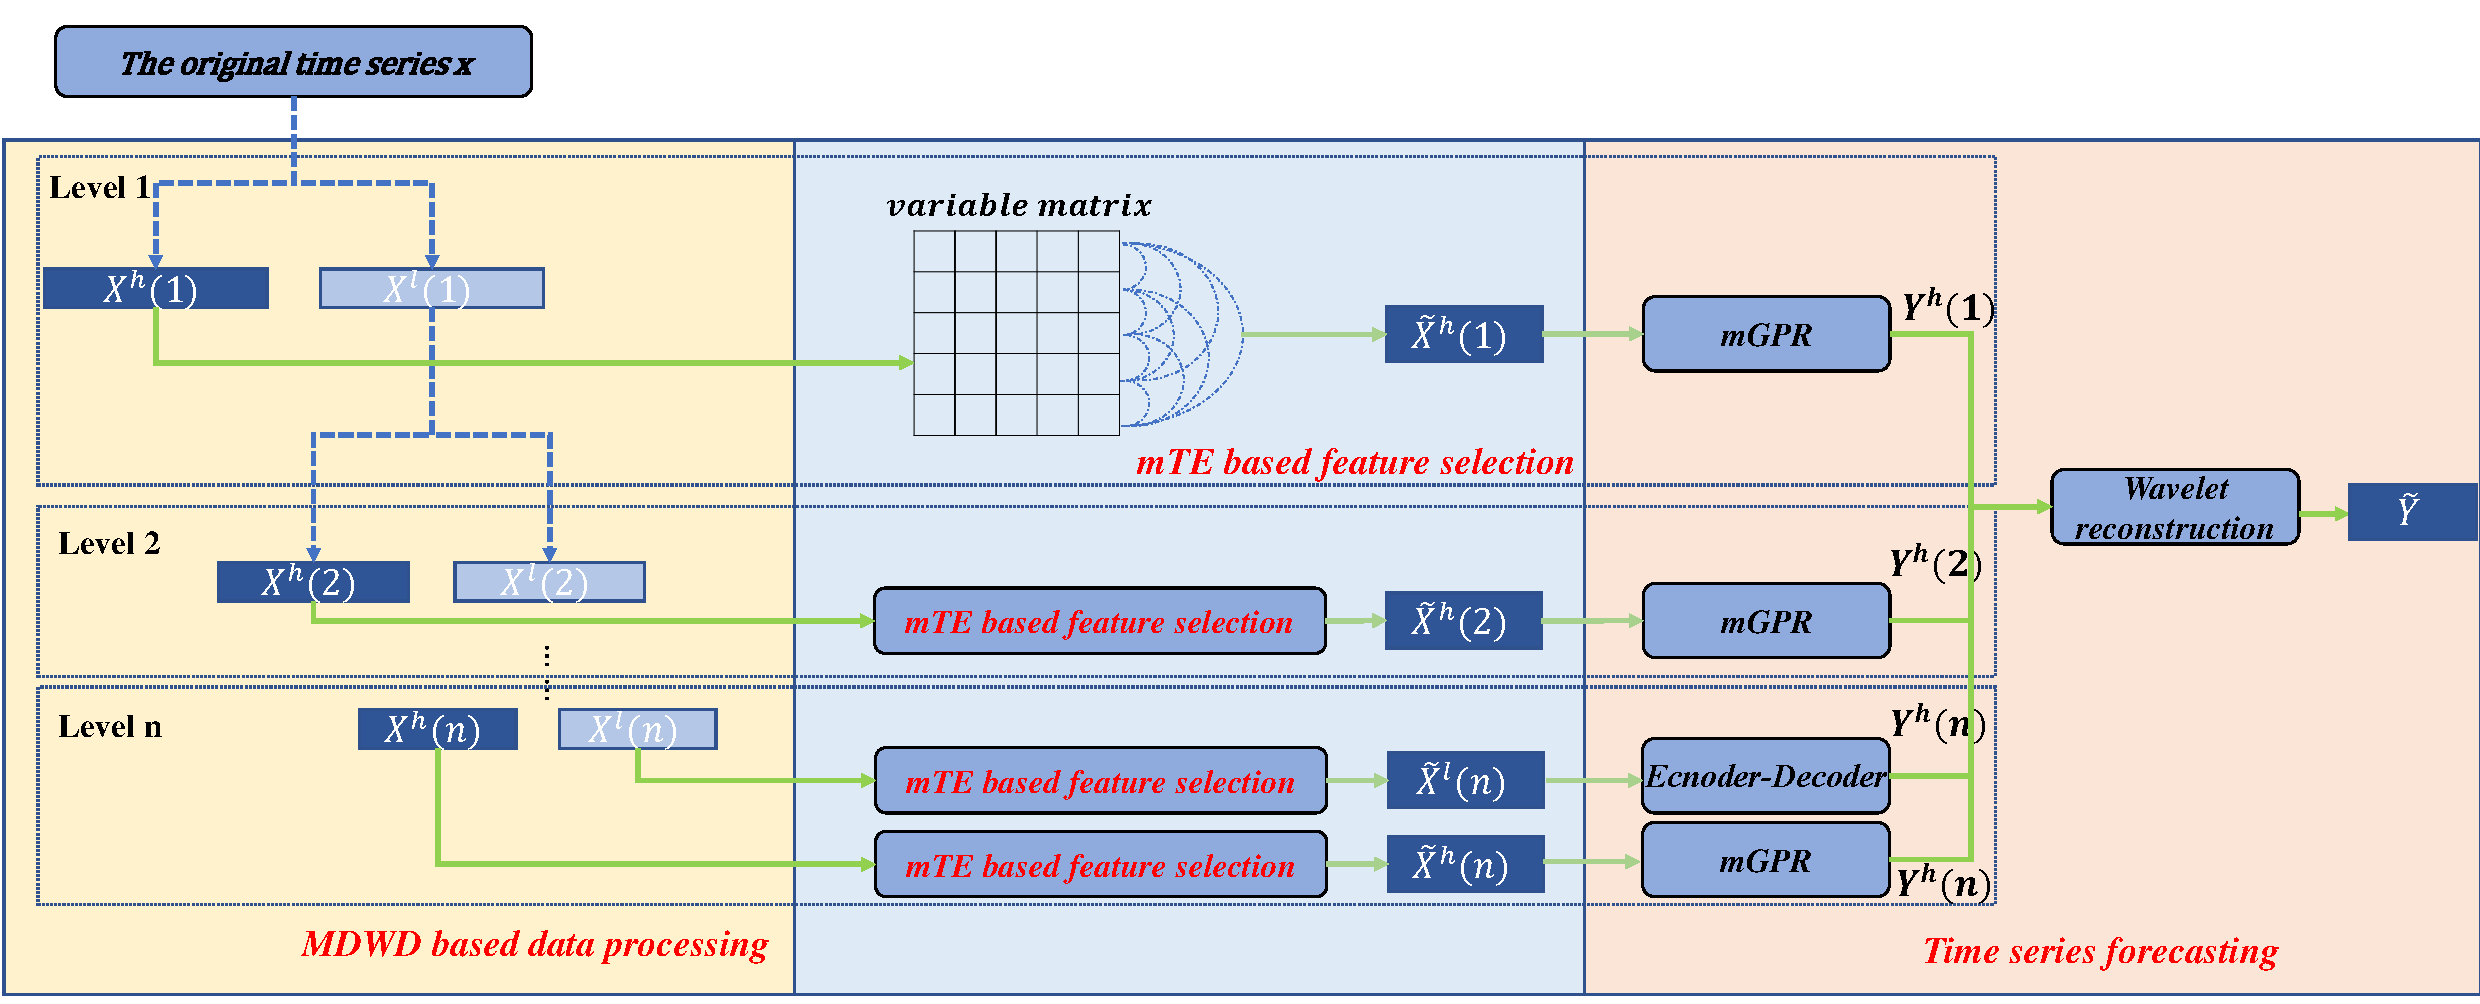
\includegraphics[scale=0.4]{./ch4/fig4_1.pdf}
\caption{基于多级小波分解和多元传递熵的时间序列分析框架示意图} \label{fig4_1}
\end{center}
\end{figure*}
所提模型的结构包括三个模块:基于 MDWD 的数据处理模块、基于 MTE 的特征选择模块和时间序列预测模块。模型的输入$X \in \mathbb{R}^{n\times T}$由$n-1$个影响因素和长度为$T$的车辙时间序列组成。输出$\tilde{Y}\in\mathbb{R}^{1\times \tau}$为沥青路面车辙预测值,其中$\tau$为预测步长。基于 MDWD 的数据处理模块将输入分解成不同的层次。每一级中的高频成分和最后一级中的低频成分作为每一级中相应的基于 MTE 的特征选择模块的输入。最后,在时间序列预测模块中,高频成分预测模型采用多元高斯过程回归模型,低频成分预测模型采用基于双向长短记忆网络(LSTM)和融合注意力机制的预测模型。

\textbf{基于 MDWD 的数据处理模块} 有关多级小波分解(MDWD)概念介绍及推导已在第二章中给出,本章不再赘述,这里只给出本章所提出框架中使用的内容。其中MDWD模块分为时间序列分解部分和重构部分,对于分解部分,给定输入时间序列 $X_{t}=x_{1},x_{2},...,x_{t}$,MDWD 在 $(i+1)$-th 层的分解输出可定义为:

\begin{equation}\label{npl1}
\begin{array}{ll}
y^{l}_{t}(i+1) = \sum_{k=1}^{K}x^{l}_{t+k-1}(i)\cdot l_{k},\\
\\
y^{h}_{t}(i+1) = \sum_{k=1}^{K}x^{l}_{t+k-1}(i)\cdot h_{k},\\
\end{array}
\end{equation}

其中,右侧的输入为第 i 层的低频序列分量 $X^{l}$ 和高频序列分量 $X^{h}$,它们是是上一层分解的子序列 $Y^{l}$ 和 $Y_{h}$ 的下采样,输出$y^{l}_{t}(i+1)$ 和$y^{h}_{t}(i+1)$ 分别是 $t$ 时间步长的低频序列分量和 $i$ 级别的高频序列分量。函数 $l_{k}$ 和 $h_{k}$ 是低通和高通滤波器的脉冲响应。从每一层的低频分量 $Y^{l}$ 和高频分量 $Y_{h}$可以重建级别 $i-1$ 的时间序列 $X$:	
\begin{equation}\label{npl1}
\begin{array}{ll}
x^{l}_{t}(i-1) = \sum_{k=1}^{K}y^{l}_{t+k-1}(i)\cdot l_{k}+\sum_{k=1}^{K}y^{h}_{t+k-1}(i)\cdot h_{k}.\\
\\
\end{array}
\end{equation}

这一过程也被称为逆离散小波变换(inverse discrete wavelet transform,IDWT)。它的过程包括向上采样和重建。变换函数 $l_{k}$ 和 $h_{k}$ 是上一级函数的缩放和移位。

\textbf{基于 MTE 的特征抽取模块} 在上一章中,我们已经介绍了一种新型的基于核函数估计的方法来计算MTE,尽管该方法具有准确性高和计算代价小的优点。但由于其本身是一种更普适性的概率密度估计方法,对于MTE中参数马尔可夫阶数$\tau$的选取并没有针对性的讨论,导致在选取$\tau$值时只能根据经验选择,会出现虚假因果关系,甚至无法发现显著因果关系。为了能够有效传递熵(effective transfer entropy, ETE),本章将继续介绍一种基于贪心算法的ETE计算方法,首先,我们回顾TE的定义,从 $Y$ 到 $X$ 的 TE 是以历史数据 $X_{t}^{k}$ 为条件,从源过程 $Y_{t}$ 到 $X$ 的实现值 $x_{\tau}$ 的条件互信息:
\begin{equation}\label{TE}
\begin{array}{ll}
T_{Y\rightarrow X}=I(Y_{t}^{k};x_{\tau} |X_{t}^{k})=-\sum^{t-k}_{i=1}\frac{log(p(x_{\tau}|x_{i},y{i}))}{p(p(x_{\tau}|x_{i}))},
\end{array}
\end{equation}

其中$Y_{t}^{k}$和$X_{t}^{k}$为长度为$k$的历史序列,$x_{\tau}$为$\tau$时刻的随机变量。$T_{Y\rightarrow X}$大于0意味着$Y$是$X$的原因。否则,$Y$就是$X$的结果。值得注意的是,TE取决于历史序列长度$k$。$T_{Y\rightarrow X}$可以表示整个概念信息传递,而$k\rightarrow \infty$。但是,$\tau$值的选取会影响TE的显著性,甚至会带来冗余信息。为了克服这些问题,\cite{31}提出了集体传递熵(CTE),它表示因果源的增量条件互信息之和:
\begin{equation}\label{npl1}
\begin{array}{ll}
T_{Y\rightarrow X}=\sum\limits_{G} I(z_{n},t;y_{t+\tau}|y_{t}^{k},z^{<n}),
\end{array}
\end{equation}
其中 $z^{<n} \in Z$ 中的 $z_{n}$ 是额外的源变量集,用于检测来自 $X$ 的冗余变量:${z^{<n}}=\{Z_{c}|\forall c: 1\leq c \leq n\}$。受 \cite{32} 的启发,我们提供了一种贪婪算法,根据 CMI 对候选变量 $C$ 的贡献从 $X$ 中选择 $Z$。算法如算法 1 所示:

\begin{algorithm}[htb]
\caption{基于贪心算法的有效传递熵(ETE)的计算}
\label{alg:SA1}
\hspace*{0.02in} {\bf 输入:} 多元源时间序列 $X$, 目标时间序列 $Y$, 相关源序列集 $Z$ and 变量历史数据候选集 $C_{X}$ and $C_{Y}$.\\
\hspace*{0.02in} {\bf 输出:} 多元因果关系集 $E$.\\
\begin{algorithmic}[1]
%\ENSURE ~~Split data set into $k$ folds $F:\{F_{1}, F_{2},..., F_{k}\}$\
\STATE Initialise $\ Z=\emptyset$,  $\ E=\emptyset$
\\

\FOR{$c \in C_{Y}$}
    \STATE $T_{c\rightarrow y_{t+ \tau}} = I(c,y_{t}|Z)$;
    \IF {$T_{c\rightarrow y_{t+ \tau}}$ meets $Maximum\ Statistics$}
        \STATE add $c$ to $Z$ and remove it from $C_{Y}$;
    \ELSE
        \STATE break;
    \ENDIF
\ENDFOR
\FOR{$c' \in C_{Y}$}
    \STATE $T_{c\rightarrow y_{t+ \tau}} = I(c',y_{t}|Z)$;
    \IF {$T_{c\rightarrow y_{t+ \tau}}$ meets $Maximum\ Statistics$}
        \STATE add $c'$ to $Z$ and remove it from $C_{X}$;
    \ELSE
        \STATE break;
    \ENDIF
\ENDFOR
\FOR{$z \in Z$}
    \STATE add $z$ to $Z'$;
    \STATE $T_{z\rightarrow y_{t+ \tau}} = I(Z_{X},y_{t}|Z_{Y})$;
    \IF {$T_{z\rightarrow y_{t+ \tau}}$ meets $Minimum\ Statistics$}
        \STATE remove $z$ from $Z$
    \ENDIF
\ENDFOR
\STATE $T_{Z_{X}\rightarrow y_{t+ \tau}} = I(Z_{X},y_{t}|Z_{Y})$;
\IF {$T_{Z_{X}\rightarrow y_{t+ \tau}}$ meets $omnibus \ test$}
    \STATE add $Z_{X}$ to $E$
\ENDIF
\RETURN $E$
\end{algorithmic}
\end{algorithm}


\subsection{时间序列预测模型}
在小波分解模块中,车辙及其影响因素的时间序列被分解为 3 层,其中最后一层的低频分量(0-20Hz)表示原始时间序列的趋势项,所有 3 层的高频分量(20-30Hz、30-50Hz 和 50-100Hz)表示原始时间序列的波动项。作为递归神经网络(RNN)的扩展,LSTM能够捕捉时间序列的长期依赖关系,而注意力机制的概念在近几年的深度学习,特别是神经网络领域的研究中得到了普及,它能有效捕捉输入数据不同部分之间的依赖关系,这在许多任务中都至关重要。(\cite{33}),因此也被被用于时间序列预测。因此,我们设计了一种基于融合注意力机制和LSTM的自编码器为趋势项的预测模型。此外,为了克服 RNN 模型在面对时间序列高频波动时的不敏感性,本文将基于统计理论的复杂时间序列高维非线性机器学习模型 GPR 引入到所提出的框架中,以预测波动项。本小节的其余部分将介绍这两个模型的机制。

\textbf{高斯随机过程} 高斯过程是随机变量的集合,其中任意有限个变量都具有联合高斯分布。给定一组点 $X = \{x_1,x_2,\ldots,x_t\}$,其值 $f(X)$ 完全由其均值函数 $m(X)$ 和协方差函数 $k(X,X')$指定,它们分别定义为:
\begin{equation}
\begin{aligned}
m(X)=\mathbb{E}[f(X)&], \\
k(X,X')=\mathbb{E}[(f(X)-m(X)&)(f(X')-m(X'))],
\end{aligned}
\end{equation}
其中,$f(X)$ 是高斯过程,可写成:
\begin{equation}
\begin{aligned}
f(X) \sim \mathcal{GP}(m(X), k(X,X')).
\end{aligned}
\end{equation}

用 $y$ 表示观测值,它与真实值 $f(X)$ 之间存在加性噪声。我们假设噪声服从独立、同分布的高斯分布,均值为零,方差为 $\sigma^2$:
$$\varepsilon \sim \mathcal{N}(0,\sigma^2).$$

根据 $f(X)$ 和先验分布,可以推断出在一组点 X 上产生的真值的期望值和方差。具体来说,要根据已知观测值和先验值估计真值 $f(X)$,我们需要联合分布:
\begin{equation}
\left[\begin{array}{c}
\boldsymbol{y} \\
\boldsymbol{f}^{\prime}
\end{array}\right] \sim \mathcal{N}\left(\left[\begin{array}{c}
\boldsymbol{\mu} \\
\boldsymbol{\mu}^{\prime}
\end{array}\right],\left[\begin{array}{cc}
\boldsymbol{K}(X, X)+\sigma_{n}^{2} I & \boldsymbol{K}\left(X^{\prime}, X\right) \\
\boldsymbol{K}\left(X, X^{\prime}\right) & \boldsymbol{K}\left(X^{\prime}, X^{\prime}\right)
\end{array}\right]\right),
\end{equation}

以及观测数据的联合高斯先验分布

\begin{equation}
\begin{aligned}
P(f'\mid y,X,X')=\mathcal{N}(m,C).
\end{aligned}
\end{equation}

有一些常用的协方差矩阵函数 K,通过对数似然框架中的优化,可以自适应地获得最佳超参数。函数值 $f'$(对应于测试输入 $X'$)可以通过评估点 $X$ 的估计均值 m 和估计方差 $C$ 从联合后验分布中采样:
\begin{equation}
\begin{array}{c}
\boldsymbol{m}=\boldsymbol{\mu}^{\prime}+\boldsymbol{K}\left(X, X^{\prime}\right)\left(\boldsymbol{K}(X, X)+\sigma_{n}^{2} I\right)^{-1}(\boldsymbol{y}-\boldsymbol{\mu}) \\
\boldsymbol{C}=\boldsymbol{K}\left(X^{\prime}, X^{\prime}\right)-\boldsymbol{K}\left(X, X^{\prime}\right)\left(\boldsymbol{K}(X, X)+\sigma_{n}^{2} I\right)^{-1} \boldsymbol{K}\left(X^{\prime}, X\right)
\end{array}.
\end{equation}

\subsection{主要结果}  



 
\textit{\textbf{最大的平均脉冲区间} }为了降低控制成本,构造如下的优化问题 以获得最大的平均脉冲区间:
\begin{align} 
&\quad\quad\quad\max \quad \mathcal{T}_a\label{4-2-34}\\
&\begin{array}{r@{\quad}r@{}l@{\quad}l}
{\rm s.t.} & (\ref{4-2-33})\ \text{中}\ a)-g).
\end{array}\nonumber
\end{align}
%\begin{remark} 
%显然, 优化问题  (\ref{4-2-33}) 和  (\ref{4-2-34}) 是关于 $Q$,$\tau$,$W$,$M$和 $U$ 的 LMIs 问题,使用 Matlab 中 Yalmip 工具箱很容易得到它们的最优解。注意到优化问题  (\ref{4-2-33}) 和  (\ref{4-2-34}) 都是以定理 \ref{t4-2-1} 的条件为约束条件构建起来的。作为特例,分别以推论 \ref{c4-2-1} 和 \ref{c4-2-2} 中条件为约束条件的优化问题很容易建立出来,由于方法类似,这里不再赘述。 
%\end{remark}

\subsection{数值实例}\label{ne}
考虑广义蔡氏电路,其状态方程描述如下: 
\begin{align}\label{4-2-35}\left\{
\begin{aligned}
\dot{s}_1(t)=&\tilde{\alpha}(s_2(t)-h(s_1)),\\
\dot{s}_2(t)=&s_1-s_2+s_3,\\
\dot{s}_3(t)=&-\tilde{\beta}s_2(t),
\end{aligned}
\right.
\end{align}
其中参数 $\tilde{\alpha}=9$,$ \tilde{\beta}=14.28$,且非线性函数为 $h(s_1)=m_{2r-1}s_1+\frac{1}{2}\sum\limits_{i=1}^{2r-1}(m_{i-1}-m_i)(|s_1+\tilde{c}_i|-|s_1-\tilde{c}_i|)$。 选取 $r=2$,$ m=[-\frac{1}{7};\frac{2}{7};-\frac{4}{7};\frac{2}{7}]$,$\tilde{c} = [1; 2.15; 3.6]$, 则系统 (\ref{4-2-35})  可以呈现出 3-涡卷混沌吸引子 \cite{yalcin2000experimental425},如图 \ref{f4-3} (a) 所示。 显然,系统 (\ref{4-2-35}) 可以写成鲁里叶系统的形式,其中 $f(s_1)=(1+\tilde{\delta})s_1-h(s_1)$, 
\begin{align*} A=
\left[ \begin{array}{ccc} -\tilde{\alpha}(1+\tilde{\delta})&\tilde{\alpha}&0\\
1&-1&1\\
0&-\tilde{\beta}&0
\end{array}\right],\ 
 B=
\left[ \begin{array}{cc} \tilde{\alpha}&0\\
0&0\\
0&0\\
\end{array}\right],\ 
 \tilde{D}=
\left[ \begin{array}{ccc} 1&0&0\\
0&0&0\\
\end{array}\right],
\end{align*}
\begin{figure}[!tp]
    \centering
    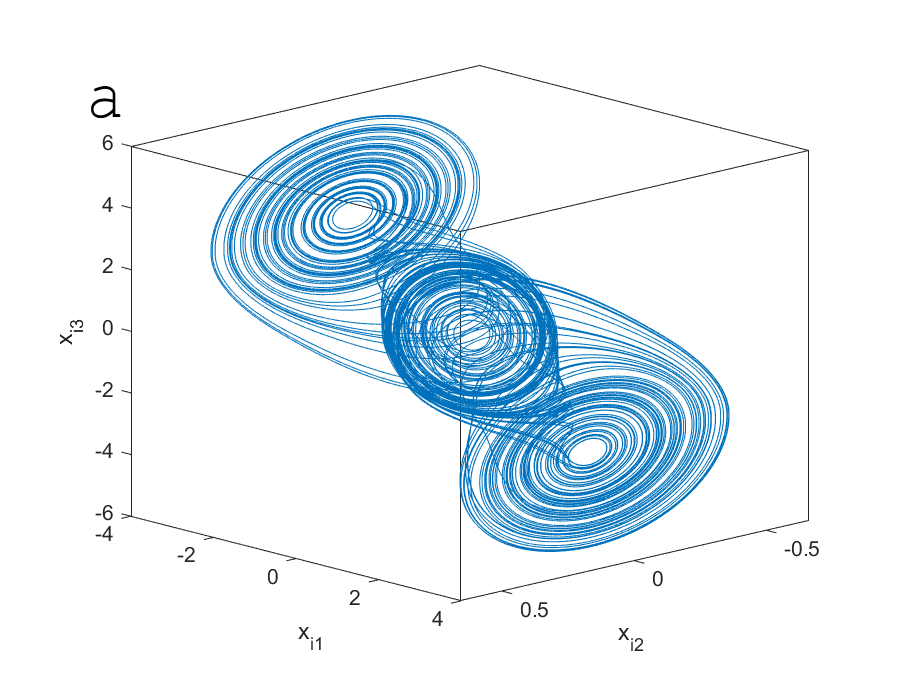
\includegraphics[scale=0.5]{./ch4/fig4-3-1.eps}
    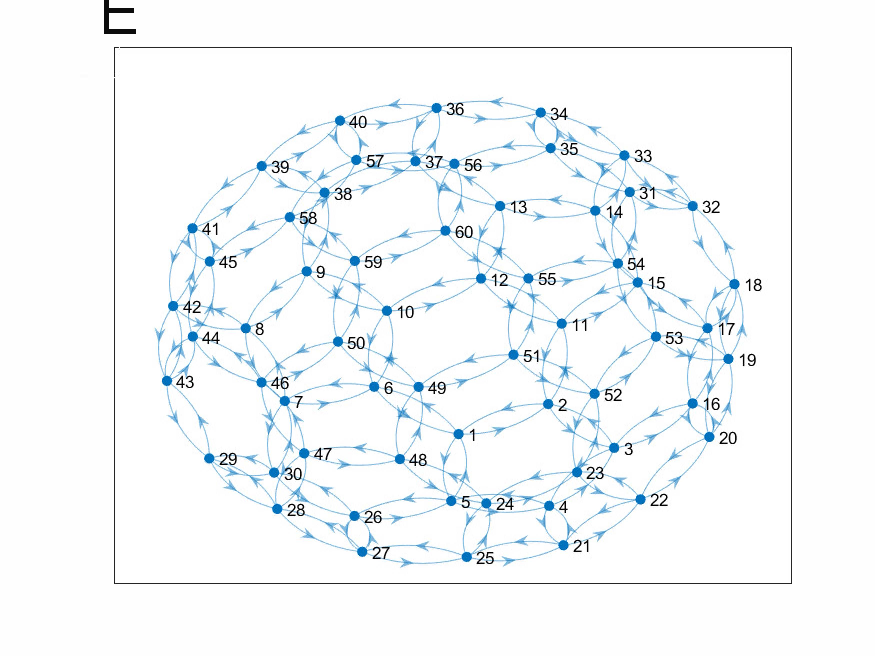
\includegraphics[scale=0.5]{./ch4/fig4-3-2.pdf} 
    \caption{(a) 3-涡卷混沌吸引子的蔡氏电路 \cite{yalcin2000experimental425}; (b) 具有 60 个节点的有向网络拓扑}
    \label{f4-3}
\end{figure}

\noindent 其中 $\tilde{\beta}=1$ 且 $f(\cdot)$ 满足扇区条件且 $l_k=2.5$,$k\in I[1,2]$。 现考虑由 $60$ 个相同的蔡氏电路系统 (\ref{4-2-35}) 耦合而成的鲁里叶网络,其中 $q(t)=\frac{1}{2}-\frac{1}{2}e^{-t}$,$ c=0.2$,$\varGamma={\rm diag}\{1,1,1\}$,且网络拓扑结构如图 \ref{f4-3} (b) 所示。

\textbf{情况一}: 选择脉冲序列为  $t_{5n-4}=0.03n-0.025$,$ t_{5n-3}=0.03n-0.017$,$ t_{5n-2}=0.03n-0.01$,$ t_{5n-1}=0.03n-0.006$,$t_{5n}=0.03n$,$n\in \mathbb{Z}_+$,容易计算出 $\mathcal{T}_{a}=0.006$。 选取形状参考集 $\chi_R=\{\varphi_1\}$, 其中 $\varphi_1= [-0.7,-0.02,0.2]^T$,通过 Yalmip 工具箱求解优化问题 (\ref{4-2-33}),可得  
 $\mu^{\text{定理 \ref{t4-3-1}}}_{opt}=0.1926$,其他的可行解为
 \begin{align*} P&=
\left[ \begin{array}{ccc} 
 2.3597&0 & 0 \\
0&   20.9991 & 2.2148\\
0&    2.2148 &   2.5951
\end{array}\right],\ 
S=
\left[ \begin{array}{ccc} 
21.2373 &0& 0\\
0 & 188.9919  & 19.9332\\
0 &  19.9332  & 23.3559
\end{array}\right],\\ 
 H&=
\left[ \begin{array}{cccccccccccc} 
0.3348&0&0\\
0&0.4281&0.0098\\
0&0&0.3349\\
0.3348&0&0\\
0&0.4200&0.0002\\
0&0&0.3349\\
0.3348&0&0\\
0&0.4200 & 0.0002\\
0  &  0& 0.3349\\
0.3348  &  0  &  0\\
0 &   0.4281 &   0.0098\\
0  &  0 &  0.3349
\end{array}\right],\\K&={\rm diag}\{0.4025,
0.4603,
0.4357\},~\overline{W}={\rm diag}\{
42.4746,
0.2894\}. 
\end{align*} 
图 \ref{f4-4}--\ref{f4-7}  是相关的数值模拟,其中图 \ref{f4-4} 展示了鲁里叶网络 (\ref{4-2-1}) 在没有脉冲控制输入的情况下是无法实现同步的,其中初始值在集合 $\mathcal{E}(\varXi\otimes P,1)$ 内随机选择。在相同的初值条件下, 通过施加分布式饱和脉冲控制,鲁里叶网络 (\ref{4-2-1}) 关于脉冲序列 $\Im(1,0.006)$ 可以实现局部指数同步,如图 \ref{f4-5} 所示。另外,如果选择初值 $\psi\in\mathcal{E}^c(\varXi\otimes P,1) \cap \mathcal{E}(\varXi\otimes P, 10/9)$,鲁里叶网络 (\ref{4-2-1}) 的局部指数同步无法实现,如图 \ref{f4-6} 所示。这些数值模拟充分证明了所得结果的可行性和有效性,并且证实了椭球 $\mathcal{E}(\varXi\otimes P,1)$ 包含在误差系统的吸引域内。 

为了表明所得结果保守性更小, 在优化问题 (\ref{4-2-33}) 相同的初值条件下,解决以推论 \ref{c4-2-1} 条件为约束条件的优化问题,可得 $\mu^{\text {推论 \ref{c4-2-1}}}_{opt}=0.0657$。 由于 $0.1926>0.0657$,这意味着定理 \ref{t4-2-1} 可以获得比推论 \ref{c4-2-1} 更大的吸引域估计, 相应的 Lyapunov 函数水平集绘于图 \ref{f4-7}。这也充分说明引理 \ref{l4-2-1} 中最新的凸包表示法在处理饱和脉冲控制约束方面比引理 \ref{l4-2-2} 具有更小的保守性。

\textbf{情况二}:
为了降低控制成本,构造了优化问题 (\ref{4-2-34})。 在情况一相同的条件下,通过求解优化问题 (\ref{4-2-34}) 可以得到最大平均脉冲区间 $\mathcal{T}_{a\_opt}=0.0071$。 因此,只要 $\mathcal{T}_{a\_opt}=0.0071$,脉冲间隔  $t_{k+1}-t_{k},\ k\in\mathbb{Z}_+$ 的上下界将不再有任何限制,允许不规则脉冲信号的存在,即脉冲间隔的上下界可以尽可能大,也可以尽可能小。因此,所得结果比文献 
\cite{wang2016impulsive1560,Rakkiyappan2017Exponential217,zhang2013synchronization,yang2007stability1448,li2020impulsive,li2020impulsivePolytopic} 中的结果具有更小的保守性。  


\begin{figure}[H]
    \centering
    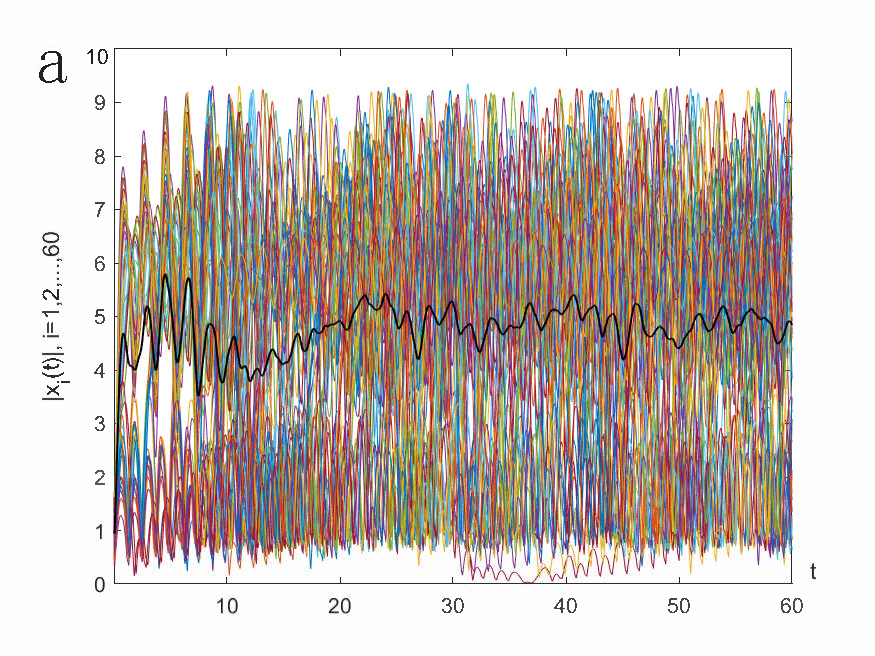
\includegraphics[scale=0.5]{./ch4/fig4-4-1.pdf}
    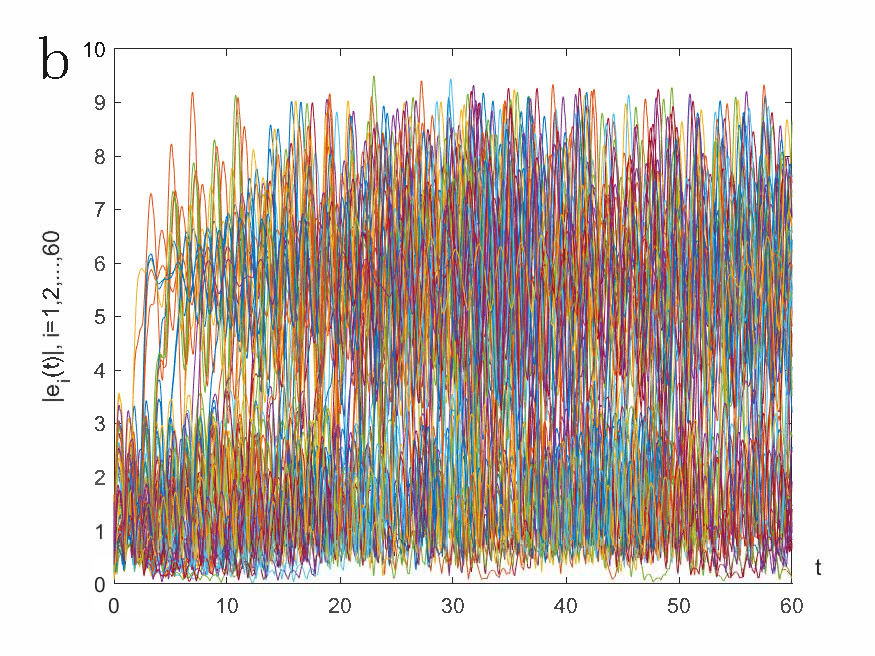
\includegraphics[scale=0.5]{./ch4/fig4-4-2.pdf}
    \caption{无脉冲下无法实现局部同步。 (a) 鲁里叶网络 (\ref{4-2-1}) 的状态轨迹;(b) 误差系统 (\ref{4-2-5}) 的状态轨迹 } 
    \label{f4-4} 
\end{figure}         
\begin{figure}[H]
    \centering
    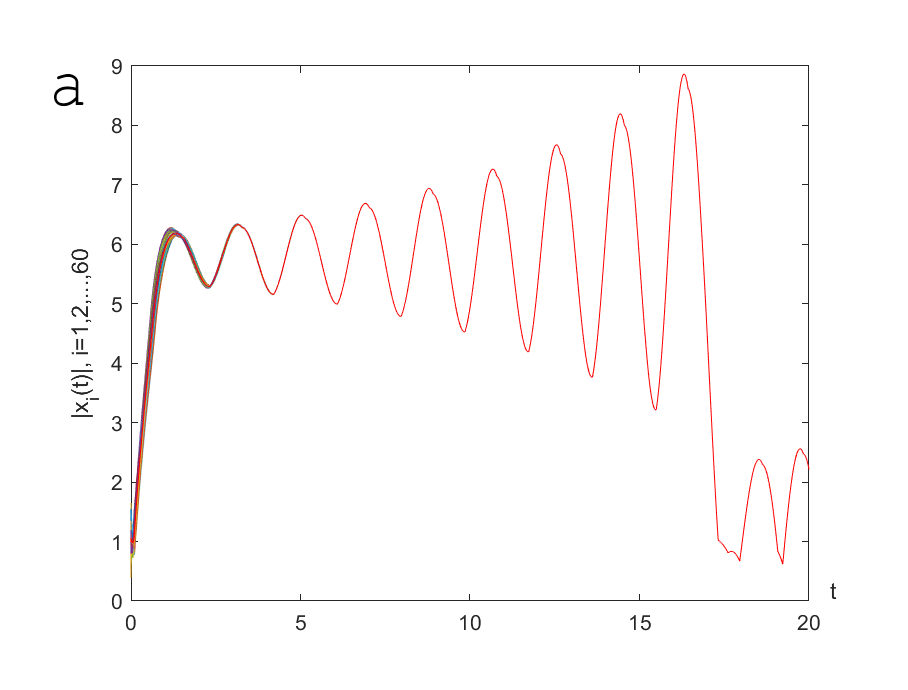
\includegraphics[scale=0.5]{./ch4/fig4-5-1.eps}
    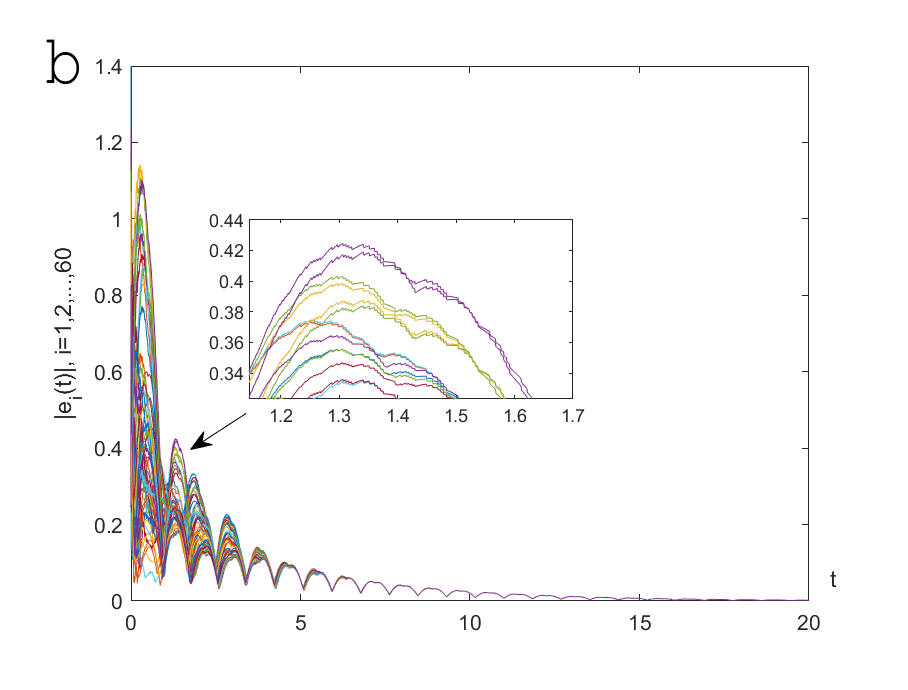
\includegraphics[scale=0.5]{./ch4/fig4-5-2.eps}
   \caption{在满足脉冲序列 $\Im(1,0.006)$ 的分布式饱和脉冲控制下可以实现局部同步。 (a) 鲁里叶网络 (\ref{4-2-1}) 的状态轨迹;(b) 误差系统 (\ref{4-2-5}) 的状态轨迹 } 
      \label{f4-5} 
\end{figure} 

\begin{figure}[H]
    \begin{center}
        \begin{minipage}[c]{0.5\textwidth}
            \centering
            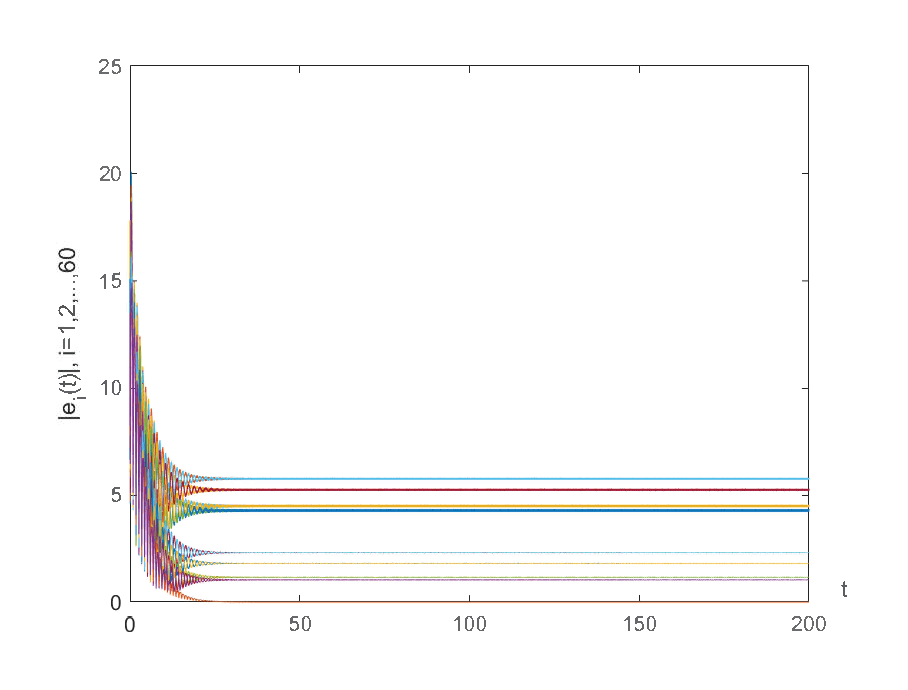
\includegraphics[scale=0.5]{./ch4/fig4-6.eps}
            \centering
            \caption{具有饱和脉冲控制且初值\\ $\psi\in\mathcal{E}^c(\varXi\otimes P,1) \cap \mathcal{E}(\varXi\otimes P, 10/9)$ \\的误差系统 (\ref{4-2-5}) 的状态轨迹}
            \label{f4-6}
        \end{minipage}%
        \begin{minipage}[c]{0.5\textwidth} \centering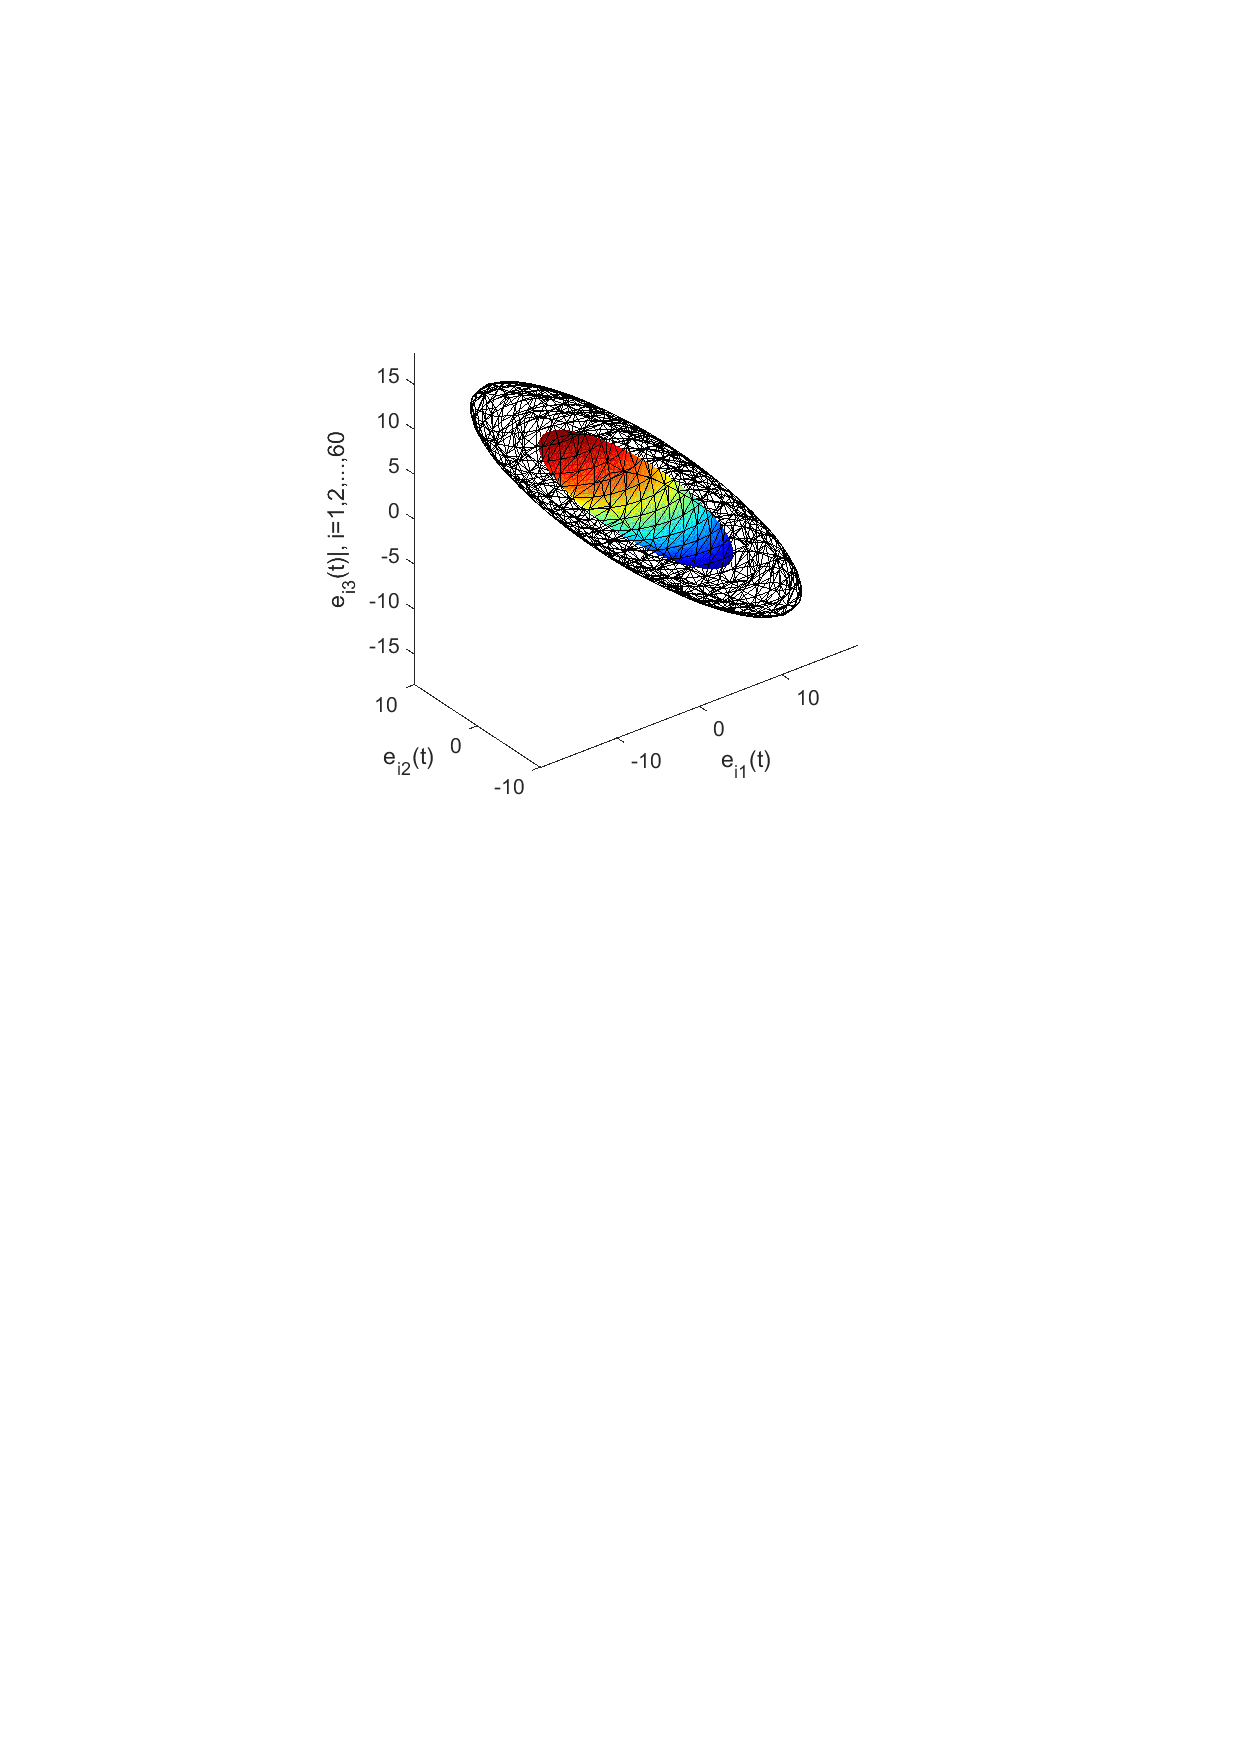
\includegraphics[scale=0.7]{./ch4/fig4-7.pdf} \vspace{0.5cm}
            \caption{基于不同方法的吸引域估计。 内部彩色椭球表示基于推论 \ref{c4-2-1} 估计的吸引域,外部黑色网格椭球表示基于定理 \ref{t4-2-1} 估计的吸引域}
            \label{f4-7}
        \end{minipage}
    \end{center}
\end{figure}
\section{分布式饱和脉冲控制下非线性时滞多智能体系统的局部一致性}
上一节开发了一种新的估计吸引域的方法,本节将在此方法的基础上继续研究分布式饱和脉冲控制下具有切换拓扑的 非线性时滞多智能体的局部一致性。为了进一步降低保守性,构造全新的复合的 Lyapunov 函数替代一般的二次 Lyapunov 函数,以估计出最接近真实的吸引域。
\subsection{模型描述}
考虑由一个领导者和 $N$ 个跟随者组成的非线性时滞多智能体系统,其动态方程为 
\begin{align}\label{4-3-1}
\left\{\begin{aligned} 
\dot{x}_0(t)=&Ax_0(t)+Bf(x_0(t-\tau(t))),\\
\dot{x}_i(t)=&Ax_i(t)+Bf(x_i(t-\tau(t)))+u_i(t),
\end{aligned}\right.
\end{align}
其中$x_0(t)$、$x_i(t)\in \mathbb{R}^n$,$i\in I[1,N]$ 分别表示领导者和第 $i$ 个跟随者的状态,$A$、$ B\in\mathbb{R}^{n\times n}$ 是已知的常矩阵,$\tau(t)$ 是时变时滞且满足 $0\leq\tau(t)\leq \tau$,这里 $\tau>0$ 是给定常量,$f(\cdot)\in \mathcal{C}^1( \mathbb{R}^n,\mathbb{R}^n) $ 是向量值非线性函数,$u_i(t)$ 表示分布式饱和脉冲控制输入,其设计如下:
\begin{align}\label{4-3-2}
u_i(t)=\sum\limits_{k=1}^{\infty}{\rm sat}(w_i(t)) \delta (t-t_k),\ k\in\mathbb{Z}_+,
\end{align}
其中 ${\rm sat}(w_i(t))=({\rm sat}( w_{i1}(t)), {\rm sat}( w_{i2}(t)),\cdots,{\rm sat}( w_{in}(t)))^T$ 是向量值饱和函数,这里 ${\rm sat}( w_{ir}(t))={\rm sgn}  (w_{ir}(t))\min\{1,|w_{ir}(t)|\}$,$r \in I[1,n]$,且 
\begin{align*}
\omega_i(t)=F\Big(\sum\limits_{j\in \mathcal{N}_i}a^{\sigma(t)}_{ij}(x_j(t)-x_i(t))+b^{\sigma(t)}_i(x_0(t)-x_i(t))\Big),
\end{align*}
其中 $F\in\mathbb{R}^{n\times n}$ 是分布式饱和脉冲控制的增益矩阵,$\sigma(t): [0,+\infty)\rightarrow
I[1,\hbar]:=\mathfrak{H}$ 为右连续的分段常数函数被称为切换信号,$\delta(\cdot)$ 是狄拉克函数,$t_k$ 是脉冲时刻,其满足 
$ 0\leq t_0<t_1<t_2<\cdots<t_k<\cdots$, 且 $\lim_{k \rightarrow+\infty}t_k=+\infty$。

定义 $z_i(t)=x_i(t)-x_0(t)$,$i\in I[1,N]$ 为第 $i$ 个跟随者和领导者之间的状态误差,在控制器  (\ref{4-3-2}) 作用下,误差系统满足 
\begin{align}\label{4-3-3}
\left\{
\begin{aligned}  
&\dot{z}_i(t)=Az_i(t)+Bf(z_i(t-\tau(t)),\ t\neq t_k,\  t\geq t_0,\\
&\Delta z_i(t_k)={\rm sat}\Big[F\Big(\sum\limits_{j\in \mathcal{N}_i} a^{\sigma(t_k)}_{ij}(z_j(t^-_k)-z_i(t^-_k)) -b^{\sigma(t_k)}z_i(t^-_k)\Big)\Big],\ k\in \mathbb{Z}_+,
\end{aligned}
\right.
\end{align}
其中 $\sigma(t_k)\in \mathfrak{H}$,$f(z_i(t-\tau(t)))=f(x_i(t-\tau(t)))-f(x_0(t-\tau(t)))$,$\Delta z_i(t_k)=z_i(t_k)-z_i(t^-_k)$,$ z_i(t^-_k)=\lim_{t\rightarrow t^-_k}z_i(t_k)$,且  $z_i(t_k)=z_i(t^+_k)=\lim_{t\rightarrow t^+_k}z_i(t_k)$。

令 $z(t)=(z^T_1(t),z^T_2(t),\dots,z^T_N(t))^T$,$ f(z(t-\tau(t)))=(f^T(z_1(t-\tau(t))), f^T(z_2(t-\tau(t))),\ldots,f^T(z_N(t-\tau(t))))^T$, 那么误差系统 (\ref{4-3-3}) 可以写成下列紧凑的形式:
\begin{flalign*} 
\left\{
\begin{aligned} 
&\dot{z}(t)= (I_N\otimes A) z(t)+ (I_N\otimes B)  f( z(t-\tau(t))),\ t\neq t_k,\ t\geq t_0, \\ 
&\Delta z(t_k)=-{\rm sat}[(\mathcal{H}^{\sigma(t_k)} \otimes F) z(t^-_k)],\
\sigma(t_k)\in \mathfrak{H},\  k\in \mathbb{Z}_+.
\end{aligned}\right.        
\end{flalign*} 
             
\begin{remark}
所设计的控制器 (\ref{4-3-2}) 不仅考虑了执行器饱和的情况,还充分考虑了切换拓扑。在实际运行过程中,多智能体系统的网络拓扑是动态变化的。 相比固定拓扑 \cite{2014Semi2222,2017Leader327,2017Adaptive4654},具有切换拓扑的多智能体系统可以更准确地反映由外部环境变化和智能体移动等引起的智能体之间连接的变化。
\end{remark}
\begin{definition}
    令 $\mathscr{F}_0$ 表示一类脉冲序列 $\{t_k,\ k\in\mathbb{Z}_+\}$, 满足 $0\leq t_0<t_1<t_2<\cdots<t_k<\cdots$ 且 $ \lim_{k \rightarrow+\infty}t_k=+\infty$。 $\mathscr{F}_{[\vartheta_0,\vartheta_1]}\subseteq \mathscr{F}_0$ 表示一类脉冲序列,满足 
    $\vartheta_0\leq t_{k+1}-t_k\leq\vartheta_1$。
\end{definition}
\begin{definition}
    如果对每个跟随者 $i$,$i\in I[1,N]$, 存在分布式饱和脉冲控制协议 (\ref{4-3-2}),对于任意吸引域内给定的初始条件,都有 
    \begin{align*}
    \lim_{t\rightarrow \infty}|x_i-x_0|=0,\ i\in I[1,N], \end{align*}  
    则称非线性时滞多智能体系统 (\ref{4-3-1}) 关于脉冲序列  $\mathscr{F}_{[\vartheta_0,\vartheta_1]}$ 可以实现局部领导者--跟随一致性。
\end{definition} 
\begin{assumption}\label{a4-3-1}
    非线性函数 $f(\cdot)$ 满足 Lipschitz 条件,即存在对角矩阵 $L_f\in\mathbb{R}^{n\times n}$,对于任意的 $ y_1$、$y_2\in \mathbb{R}^n$,都有
    \begin{align*}
    |f(y_1)-f(y_2)|\leq| L_f(y_1-y_2)|. 
    \end{align*}
\end{assumption}
\begin{assumption}\label{a4-3-2}
    每个拓扑结构 $\bar{\mathcal{G}}^{\sigma(t_k)}$,$ \sigma(t_k)\in \mathfrak{H}$,$ k\in\mathbb{Z}_+$ 包含节点 $x_0$ 作为根节点的有向生成树。 
\end{assumption}

应用引理  \ref{l4-2-1},存在矩阵  $H\in\mathbb{R}^{\bar{n}\times n}$,如果 $|(\mathcal{H}^{\sigma(t_k)}\otimes  H)z(t^-_k)|_{\infty} \leq 1$,则有
\begin{flalign*}
{\rm sat}[(\mathcal{H}^{\sigma(t_k)} \otimes F) z(t^-_k)] 
= \sum\limits_{l=1}^{2^n}c _{l}(t_k) 
\big[\mathcal{H}^{\sigma(t_k)} \otimes (D_{l}F+\mathscr{D}^-_{l}H)\big]z(t^-_k),\ \sigma(t_k)\in \mathfrak{H},
\end{flalign*}
其中 $c_{l}(t_k)$ 是一组非负标量函数且满足 $\sum\limits_{l=1}^{2^n}c_{l}(t_k)=1$,$l\in I[1,2^n]$,$k\in\mathbb{Z}_+$。


那么误差系统 (\ref{4-3-3}) 可以进一步写成
\begin{align}\label{4-3-4}\left\{
\begin{aligned}  
&\dot{z}(t)=(I_N\otimes A) z(t)+ (I_N\otimes B)  f( z(t-\tau(t))),\ t\neq t_k,\ t\geq t_0,\\ 
&\Delta z(t_k)=-\sum\limits_{l=1}^{2^n}c     _{l}(t_k)\left[\mathcal{H}^{\sigma(t_k)} \otimes (D_{l}F+\mathscr{D}^-_{l}H)\right] z(t^-_k),\    \sigma(t_k)\in \mathfrak{H},\ k\in \mathbb{Z}_+,
\end{aligned}\right.
\end{align}
其初值条件为 
\begin{align*}z_{t_0} =\phi (\theta),\ \theta\in[-\tau,0],
\end{align*}
其中 $\phi\in\mathcal{PC}([-\tau,0],\mathbb{R}^{Nn})$  是向量值初始函数,其范数为
$\|\phi\|_{\tau}= \sup_{\theta\in[-\tau,0]}|\phi(\theta) |$。

令 $(\mathcal{H}^{\sigma(t_k)}\otimes H)_\varsigma$ 是矩阵 $(\mathcal{H}^{\sigma(t_k)}\otimes H)$ 的第 $\varsigma$ 行, $\varsigma\in I[1,N\bar{n}]$,定义如下对称多面体: 
\begin{align*}
\mathscr{L}(H)=\bigcap_{\sigma(t_k)\in \mathfrak{H}} \mathscr{L}(H)_{[\sigma(t_k)]},\ k\in \mathbb{Z}_+,
\end{align*}
其中
$\mathscr{L}(H)_{[\sigma(t_k)]}=\{z(t)\in \mathbb{R}^{Nn}:\ |(\mathcal{H}^{\sigma(t_k)}\otimes H)_\varsigma z(t)| \leq 1,\ \varsigma\in I[1,N\bar{n}]\} 
$。

\begin{lemma}\label{l4-3-1} 考虑下列饱和脉冲泛函微分方程: 
    \begin{align}\label{4-3-5}\left\{
    \begin{aligned} 
   & \dot{\chi}(t)= \mathcal{F}(t, \chi(\cdot)) ,\ t\neq t_k,\ t\geq t_0,\\ 
    &\Delta \chi(t_k)= {\rm sat}[\mathcal{J}_k(t_k, \chi(t^-_k))],\ k\in \mathbb{Z}_+,\\
    &\chi(\theta)=\psi(\theta),\ \theta\in[-\tau,t_0],
    \end{aligned}\right.
    \end{align}    
    则系统 (\ref{4-3-5}) 的解关于脉冲序列  $\mathscr{F}_{[\vartheta_0,\vartheta_1]}$,$\vartheta_1 <  \frac{\ln q}{p}$,是局部指数稳定的,
    如果对任意吸引域内的初值,存在函数 $V(t, \chi)\in v_0$,常数 $p> 0$,$q>1$,$v_1>0$,$v_2>0$,$m>0$ 和 $\gamma>0$, 使得
    \begin{itemize}
        \item[$(i)$] $v_1|\chi|^m \leq V(t, \chi) \leq v_2|\chi|^m$,对所有的 $(t, \chi)\in[t_0,+\infty)\times \mathbb{R}^n$ 都成立;
        \item[$(ii)$] 对于任意的  $\psi\in\mathcal{PC}([-\tau, t_0],\mathbb{R}^n)$,如果 $e^{\gamma \theta}V(t + \theta,\psi(\theta))\leq q V (t,\psi(0))$,$ \theta\in[-\tau, 0]$,$t \neq t_k$,那么 $D^+V(t,\psi(0))\leq p V( t,\psi(0))$;
        \item[$(iii)$] 对于所有的 $(t_k ,\psi)\in \mathbb{R}_+\times \mathcal{PC}([-\tau, 0],\mathbb{R}^n)$,有
        $$V(t_k ,\psi(0) + {\rm sat}(\mathcal{J}_k (t_k ,\psi)))\leq\frac{1}{q} V(t_k^- ,\psi(0)).$$   
    \end{itemize}
\end{lemma} 
\begin{remark}
值得注意的是引理 \ref{l4-3-1} 中的条件 $(i)$ 是文献 \cite{zhang2017sampled2199} 中引理 2.1 的条件  $(i)$ 的特殊形式,这是推导出指数稳定性的关键步骤; 条件 $(ii)$ 充分诠释了 Lyapunov-Razumikhin 方法的思想,条件 $(ii)$ 中的 $e^{\gamma\theta}$ 项包含时滞的信息,可以是有限时滞也可以是无穷时滞; 与文献 \cite{zhang2017sampled2199} 中引理不同的是,条件 $(iii)$  包含饱和脉冲控制项 ${\rm sat}(\mathcal{J}_k (t_k ,\psi))$,它为系统带来了局部特征。 在这种情况下,系统的初值不能拓展到整个状态空间,而只能包含在吸引域中。 虽然存在 差异,但引理 \ref{l4-3-1} 的证明方法与 \cite{zhang2017sampled2199} 中的引理  2.1 类似,这里省略。
\end{remark}
\subsection{主要结果}\label{cc}
\subsubsection{依赖脉冲时刻的复合型 Lyapunov 函数}
为了进一步降低保守性,受文献 \cite{2017Stability129} 启发, 本小节构造一种新颖的依赖于脉冲时刻的复合型 Lyapunov 函数。首先,将每个脉冲区间  $[t_{k-1},t_k)$, $k\in\mathbb{Z}_+$ 平均分成   $\mathcal{J}_0$ 个子区间,其长度为     $t_{k,m}-t_{k,m-1}=(t_k-t_{k-1})/\mathcal{J}_0$,$m\in I[1,\mathcal{J}_0]$,其中 $t_{k0}=t_{k-1}$,$ t_{k\mathcal{J}_0}=t_{k}$。 其次,介绍下列的分段函数 (有/无时滞):
\begin{flalign*}
\varGamma_{10}(t)=&\left\{ 
\begin{aligned}
&\frac{t-t_{k,m-1}}{t_{k,m}-t_{k,m-1}},\ t\in[t_{k,m-1},t_{k,m}),\\
&1,\ t\in[t_0-\tau,t_0),
\end{aligned}\right.~
\varGamma_{20}(t)=\left\{ 
\begin{aligned}
&\varGamma_{10}(t-\tau(t)),\ t-\tau(t)\in [t_0,+\infty),\\
&1,\ t-\tau(t)\in [t_0-\tau,t_0),
\end{aligned}\right.\\
\varGamma_{30}(t)=& \left\{ \begin{aligned}
&\frac{\alpha(t)-\tilde{\eta}_{m-1}}{\tilde{\eta}_{m}-\tilde{\eta}_{m-1}},\ \eta_{m}\neq 1,\\
&\tilde{\eta}_{m-1},\ \eta_{m}=1,
\end{aligned}\right.~
\varGamma_{40}(t)=\left\{ 
\begin{aligned}
&\frac{\beta_k-1/\vartheta_1 }{1/\vartheta_0 -1/\vartheta_1},\  \vartheta_0<\vartheta_1,\\
&1/\vartheta_0,\ \vartheta_0=\vartheta_1,
\end{aligned}\right.\\ \varGamma_{j1}(t)=&1-\varGamma_{j0}(t),\ j\in I[1,4],
\end{flalign*}
其中 $\alpha(t)= \tilde{\eta}_{m-1}\eta^{\varGamma_{10}(t)}_m$,$ \tilde{\eta}_{m}=\prod\limits_{i=1}^{m}\eta_i$,$ \tilde{\eta}_{0}=1$,$\eta_m\in \mathbb{R}_+,\ m\in I[1,\mathcal{J}_0]$,$\beta_k=
1/(t_k-t_{k-1})$,$k\in\mathbb{Z}_+$。\\
基于此,构造下列依赖于脉冲时刻的复合型 Lyapunov 函数: 
\begin{align} \label{4-3-6}
V(t,z(t))=\sum\limits_{i=1}^{N} \alpha(t)z^T_i(t)P(t)z_i(t),\ t\in [t_{k,m-1},t_{k,m}),\  m\in I[1,\mathcal{J}_0],\ k\in\mathbb{Z}_+, 
\end{align} 
其中 $P(t)=\sum\limits_{r=0}^{1}\varGamma_{1r}P_{m-r},\ P_{j}>0$,$j\in I[0,\mathcal{J}_0]$。 

 
定义 $V(t,z(t))$ 的一个水平集: $$ \mathscr{E} ( P(t),1)=\{z(t)\in \mathbb{R}^{Nn}:\  V(t,z(t))\leq 1\}.$$

\begin{remark} 
为了降低保守性,设计了非二次的时变 Lyapunov 函数 (\ref{4-3-6}),显然它依赖于脉冲时刻且包含由几个正定矩阵 $P_0$,$P_1$,$\cdots$,$P_{\mathcal{J}_0}$ 组成的凸包,这导致更多的决策变量可以被引入到随后建立的优化问题,使所得的结果保守性更小。 相比二次 Lyapunov 函数  \cite{2013Analysis871,2014Global499,2017Global1270,2020Performance734,2013Adaptive1545,2018Event4391,2020Consensus194,2020Adaptive3013960},基于依赖于脉冲时刻的复合型 Lyapunov 函数来估计吸引域可以缩短与真实吸引域的差距,更易获得最大的吸引域估计。
\end{remark}

\subsubsection{切换拓扑下局部领导者--跟随一致性} 
\begin{theorem}\label{t4-3-1} 
    在假设 \ref{a4-3-1} 和假设 \ref{a4-3-2} 成立的条件下,具有切换拓扑的非线性时滞多智能体系统 (\ref{4-3-1}) 关于脉冲序列 $\mathscr{F}_{[\vartheta_0,\vartheta_1]}$ 可以实现局部领导者--跟随一致性,如果存在 $n\times n$ 矩阵组 $P_{j}>0$,$j\in I[0,\mathcal{J}_0]$, 和正标量 $p$,$q>1$,$\gamma$,$ \mu_{1rgs\hslash}$, $\mu_{2\hslash}$,这里 $r$、$g$、$s$、$\hslash\in I[0,1]$ 使得下列的不等式成立: 
    \begin{align}\label{4-3-7} 
    \left[ \begin{array}{cc}
    -\frac{1}{q}&  (\mathcal{H}^{\sigma(t_k)}\otimes H)_\varsigma\\
    \star&-\check{\eta}_{ms}I_N\otimes P_{m-r}  \\
    \end{array}
    \right]\leq 0,\ \varsigma\in I[1,N\bar{n} ], 
    \end{align} 
    \begin{align} \label{4-3-8} 
    &\left[ \begin{array}{cc}
    -\frac{\tilde{\eta}_{J_0}}{q}I_N\otimes P_{\mathcal{J}_0}& \varPsi_{l}\\
    \star&-I_N\otimes P_0
    \end{array}
    \right]\leq0,\ l\in I[1,2^n],
    \end{align}
    \begin{align}\label{4-3-9} 
    \varOmega_{rgs\hslash}= \left[ \begin{array}{ccc}
    \varOmega_{11rs\hslash} &0& \check{\eta}_{ms}P_{m-r}B \\
    \star&\varOmega_{22rgs\hslash} &0 \\
    \star&\star&-\mu_{1rgs\hslash                            }I_n  
    \end{array}
    \right]< 0,
    \end{align} 
    \begin{align}\label{4-3-10} 
    \vartheta_1<\frac{\ln q}{p},
    \end{align} 
    其中 $ \varPsi_{l}= [I_{Nn}- \mathcal{H}^{\sigma(t_k)} \otimes (D_{l}F+\mathscr{D}_{l}^-H)\big]^T(I_N\otimes P_0)$,$    
    \varOmega_{11rs\hslash}= 
     \check{\eta}_{ms}[\frac{\mathcal{J}_0 \ln \eta_m}{\vartheta_{\hslash}} P_{m-r}+P_{m-r}A+A^TP_{m-r}+\frac{\mathcal{J}_0}{\vartheta_{\hslash}} (P_m-P_{m-1})-p P_{m-r}]
    +\mu_{2\hslash} qP_{m-r}$,$  
    \varOmega_{22rgs\hslash}= \mu_{1rgs\hslash}L^T_f L_f-\mu_{2\hslash}
    e^{-\gamma\tau}\varpi(\eta_{ms})P_{m-g},\ 
    \check{\eta}_{ms}=\tilde{\eta}_{m-1}\eta^{1-s}_{m}$,$ m\in I[1,\mathcal{J}_0]$,$
    \varpi(\eta_{ms})= \left\{ \begin{aligned}
     &1/\eta^{1-s}_{m},\ \eta_{m}\in[1,+\infty),\\ 
     &\eta^{1-s}_{m},\ \eta_{m}\in(0,1).\end{aligned}\right.
$ 并且, 水平集 $ \mathscr{E} ( P(t),1)$ 包含在误差系统 (\ref{4-3-4}) 的吸引域内。
\end{theorem}

\begin{proof}
    假设 $z(t):=z(t,t_0,\phi)$ 是系统 (\ref{4-3-4})  过点 $(t_0,\phi)$ 的解。 通过计算, $\alpha(t)$ 可以重新表示为 $\alpha(t)=\sum\limits_{s=0}^{1}\varGamma_{3 s}(t)\check{\eta}_{ms}$,$m\in I[1,\mathcal{J}_0]$, 则条件 (\ref{4-3-7}) 等价于
    \begin{align*} 
    \left[ \begin{array}{cc}
    -\frac{1}{q}&  (\mathcal{H}^{\sigma(t_k)}\otimes H)_\varsigma\vspace{0.2cm}\\
    \star&- \alpha(t)I_N\otimes  P(t)   \\
    \end{array}
    \right]\leq 0,\ \varsigma\in I[1,N\bar{n} ],
    \end{align*} 
    这意味着 
    $\mathscr{E} ( P(t),q)\subseteq \mathscr{L}(H)$。  现在宣称,对任意的初值 $\phi\in \mathscr{E}( P(t),1)$ 都有 
    \begin{align}\label{4-3-11} z(t)\in \mathscr{E}(P(t),q),\ t\geq t_0.
    \end{align} 
    如若不然,则存在 $\check{t}>t_0$, 有 $z(\check{t})\in \mathscr{E}^c( P(t),q)$。  为了方便起见,令 $V(t):= V(t,z(t))$。  因为 $q>1,$ 所以 $ V(t_0)<q<V(\check{t}) $。定义 $\hat{t}=\sup\{t\in(t_0,\check{t})|z(t)\in \mathscr{E}( P(t),q)\}$, 有 $V(\hat{t})=q$ 且
    \begin{align}\label{4-3-12}
    V(\hat{t})<V(t)\leq V(\check{t}),\ \forall t\in(\hat{t},\check{t}].
    \end{align}
    
    当 $ t=t_k$,$k\in\mathbb{Z}_+ $ 时,基于 $P(t)$ 和 $\alpha(t)$ 的定义,则有 
    $P(t_k)=P_0$,$P(t^-_k)=P_{\mathcal{J}_0}$,$ \alpha(t_k)=1$, 且 $\alpha(t^-_k)=\tilde{\eta}_{J_0}$。 由 (\ref{4-3-8}) 和 引理 \ref{l1-3-6} 可得  
    \begin{align*} 
    &\left[ \begin{array}{cc}
    -\frac{\tilde{\eta}_{J_0}}{q}I_N\otimes P_{\mathcal{J}_0}& \varPsi_{l}\vspace{0.2cm}\\
    \star&-I_N\otimes P_0
    \end{array}
    \right]\leq0 \\
    \Leftrightarrow& \left[ \begin{array}{cc}
    I_n\otimes I_N& [I_{Nn}- \mathcal{H}^{\sigma(t_k)} \otimes (D_{l}F+\mathscr{D}_{l}^-H)]^T\vspace{0.2cm}\\
    \star&I_n\otimes I_N
    \end{array}\right]\left[ \begin{array}{cc}
    -\frac{\tilde{\eta}_{J_0}}{q}I_N\otimes P_{\mathcal{J}_0}& \varPsi_{l}\vspace{0.2cm}\\
    \star&-I_N\otimes P_0
    \end{array}
    \right]\\
    &\times\left[ \begin{array}{cc}
    I_n\otimes I_N& 0\vspace{0.2cm}\\
    I_{Nn}- \mathcal{H}^{\sigma(t_k)} \otimes (D_{l}F+\mathscr{D}_{l}^-H)&I_n\otimes I_N
    \end{array}\right]\leq0\\ 
    \Leftrightarrow& \left[ \begin{array}{cc}
    \acute{\varPsi}_{l}& 0\vspace{0.2cm}\\
    \star&-I_N\otimes P_0
    \end{array}\right]\leq0\\ 
    \Leftrightarrow& 
    \ \acute{\varPsi}_{l}
    \leq 0, 
    \end{align*}
    其中 $\acute{\varPsi}_{l}= -\frac{\tilde{\eta}_{J_0}}{q}(I_N\otimes P_{\mathcal{J}_0})+[I_{Nn}- \mathcal{H}^{\sigma(t_k)} \otimes (D_{l}F+\mathscr{D}_{l}^-H)\big]^T(I_N\otimes P_0)[I_{Nn}- \mathcal{H}^{\sigma(t_k)} \otimes (D_{l}F+\mathscr{D}_{l}^-H)\big]$, 这意味着
    \begin{align}\label{4-3-13}
    \begin{split}
    V(t_k)
    =&\alpha(t_k)z^T(t_k)(I_N\otimes P(t_k))z(t_k)\\
    =&z^T(t^-_k)\sum\limits_{l=1}^{2^n}c_{l}(t_k)\Big\{\big[I_{Nn}- \mathcal{H}^{\sigma(t_k)} \otimes (D_{l}F+\mathscr{D}_{l}^-H)\big]^T ( I_N\otimes P_0)\\
    &\times\big[I_{Nn}- \mathcal{H}^{\sigma(t_k)} \otimes (D_{l}F+\mathscr{D}_{l}^-H)\big]\Big\}z(t^-_k)\\
    \leq&\frac{\tilde{\eta}_{J_0}}{q}z^T(t^-_k) (I_N\otimes P_{\mathcal{J}_0})z(t^-_k)\\
    =&\frac{1}{q} V(t^-_k),
    \end{split}
    \end{align}
    结合 $\hat{t}$ 的定义和 $q>1$,可以验证  $\hat{t}$ 是非脉冲时刻。\\
   另一方面,取 
    $P(t-\tau(t))=\sum\limits_{g=0}^{1}\varGamma_{2 g}(t) P_{m-g}$,$\beta_k = \sum\limits_{\hslash=0}^{1}\frac{\varGamma_{4 \hslash}(t) }{ \vartheta_\hslash}$,$\mu_1(t)= \sum\limits_{r,g,s,\hslash=0}^{1}\varGamma_{1 r}(t)\varGamma_{2g}(t)\\\varGamma_{3s}(t)\varGamma_{4\hslash}(t)\mu_{1rgs\hslash}$,$  \mu_2(t)=\sum\limits_{\hslash=0}^{1} \varGamma_{4\hslash}(t) \mu_{2\hslash}$,$\varOmega (t)=\sum\limits_{r,g,s,\hslash=0}^{1}\varGamma_{1 r}(t)\varGamma_{2g}(t)\varGamma_{3s}(t)\varGamma_{4\hslash}(t) \varOmega_{rgs\hslash}$,那么 (\ref{4-3-9}) 等价于
    \begin{align}\label{4-3-14} 
    \varOmega (t)= \left[ \begin{array}{ccc}
    \varOmega_{11}(t) &0&  \alpha(t)P(t)B \vspace{0.2cm}\\
    \star&\varOmega_{22}(t) &0 \vspace{0.2cm}\\
    \star&\star& -\mu_1(t)I_n\\
    \end{array}
    \right]< 0,
    \end{align}
    其中
    $
    \varOmega_{11}(t)= \alpha(t)[\mathcal{J}_0\beta_{k}\ln \eta_mP(t)+P(t)A+A^TP(t) +\mathcal{J}_0\beta_{k}(P_m-P_{m-1})-p P(t)]
    +\mu_2(t)qP(t)$,$
    \varOmega_{22}(t)= \mu_1(t)L^T_f L_f-\mu_2(t)
    e^{-\gamma\tau}\varpi(\eta_{ms}) P(t-\tau(t))  
    $。
    
    考虑依赖于脉冲时刻的复合型 Lyapunov 函数 (\ref{4-3-6}),计算 $V(t)$ 沿着系统 (\ref{4-3-4}) 的轨迹关于 $t\in[t_{k,m-1},t_{k,m})$,$k\in\mathbb{Z}_+$,$m\in I[1,\mathcal{J}_0]$ 的右上 Dini 导数,可得 
    \begin{flalign}\label{4-3-15}
    \begin{split}
    D^+V(t)=&\alpha(t)\sum\limits_{i=1}^N [z^T_i(t)(\mathcal{J}_0\beta_{k}\ln \eta_mP(t)+P(t) A+A^TP(t)\\
    &+\mathcal{J}_0\beta_{k}(P_m-P_{m-1}))z_i(t) +2 z^T_i(t)P(t)Bf(z_i(t-\tau(t)))].
    \end{split}
    \end{flalign} 
    根据假设 \ref{a4-3-1},有
    \begin{align*}
    f^T(z_i(t-\tau(t))) f(z_i(t-\tau(t)))
    \leq \ z^T_i(t-\tau(t)) L^T_fL_f z_i(t-\tau(t)), 
    \end{align*}
    这意味着
    \begin{align}\label{4-3-16} 
    \mu_1(t)\sum\limits_{i=1}^N \big[ z^T_i(t-\tau(t))  L^T_fL_f z_i(t-\tau(t)) - f^T(z_i(t-\tau(t)))f(z_i(t-\tau(t)))\big]\geq 0.
    \end{align}
    考虑到引理 \ref{l4-3-1} 的条件 $(ii)$,当  
    $
    e^{\gamma s}V(t+s,\phi(s))\leq q V (t,\phi(0))
    $ 时,
 下式成立:
    \begin{align}\label{4-3-17} 
    \mu_2(t)\sum\limits_{i=1}^N \big[qz^T_i(t)P(t)z_i(t )
    -e^{-\gamma\tau}\varpi(\eta_{ms} )  z^T_i(t-\tau(t))P(t-\tau(t))z_i(t-\tau(t))\big]\geq 0.
    \end{align} 
    将 (\ref{4-3-16}) 和 (\ref{4-3-17}) 代入到 (\ref{4-3-15}) 中,可得 
    \begin{align*}  
    D^+V(t)-p V(t) \leq\sum\limits_{i=1}^N   \zeta^T_{i}(t)\varOmega (t)\zeta_{i}(t), 
    \end{align*} 
    其中 $\zeta_{i}=[z^T_i(t), z^T_i(t-\tau(t)),  f^T(z_i(t-\tau(t)))]^T$。那么,由  (\ref{4-3-14}) 可得 
    \begin{align}\label{4-3-18} 
    D^+V(t)\leq p V(t).
    \end{align} 
    显然,(\ref{4-3-6})、(\ref{4-3-10})、(\ref{4-3-13}) 和 (\ref{4-3-18}) 满足引理 \ref{4-3-1} 所有的条件,因此 
    \begin{align*}
    V(t)\leq  q  V(t_0) e^{-\gamma(t-t_0)},  
    \end{align*}
    这意味着对任意的 $\phi\in \mathscr{E}( P(t),1)$,存在 $\check{t}>\hat{t}$, 使得 
   $
    V(\check{t})\leq q= V(\hat{t})  
 $,
    这与 (\ref{4-3-12}) 矛盾,所以 (\ref{4-3-11}) 成立得证。 由此可得
    \begin{align*}
    |z(t)|\leq\sqrt{\frac{q\lambda_1 }{\lambda_0\bar{\varpi} } }\|\phi\|_{\tau}e^{-\frac{\gamma}{2} (t-t_0)}\rightarrow 0,\ t \rightarrow +\infty,
    \end{align*}
    其中 $\bar{\varpi}= \min\{\lambda_{\min}( \varpi(\eta_{ms}))$,$m\in I[0,\mathcal{J}_0]$,$s\in I[0,1]\}$,$\lambda_0=\min\{\lambda_{\min}(P_m)$,$m\in I[0,\mathcal{J}_0]\}$, $\lambda_1=\max\{\lambda_{\max}(P_m)$,$m\in I[0,\mathcal{J}_0]\}$。  
   则具有切换拓扑的非线性时滞多智能体系统 (\ref{4-3-1}) 关于脉冲序列 $\mathscr{F}_{[\vartheta_0,\vartheta_1]}$ 可以实现局部领导者--跟随一致性。并且, 水平集 $ \mathscr{E} ( P(t),1)$ 包含在误差系统 (\ref{4-3-4}) 的吸引域内。证毕。 
\end{proof}
 
特别的,当 $\mathscr{D}^-_{l}=D^-_l$,$l\in I[1,2^n]$。 基于引理 \ref{l4-2-2},存在矩阵 $\tilde{H}\in\mathbb{R}^{n\times n}$,如果 $|(\mathcal{H}^{\sigma(t_k)}\otimes  \tilde{H})z(t^-_k)|_{\infty} \leq 1$,那么
\begin{flalign}\label{4-3-19} 
{\rm sat}[(\mathcal{H}^{\sigma(t_k)} \otimes F) z(t^-_k)]
= \sum\limits_{l=1}^{2^n}c _{l}(t_k) 
\big[\mathcal{H}^{\sigma(t_k)} \otimes (D_{l}F+D^-_{l}\tilde{H})\big]z(t^-_k),\ \sigma(t_k)\in \mathfrak{H}. 
\end{flalign} 

基于定理 \ref{t4-3-1} 和 (\ref{4-3-19}),有以下推论。 
\begin{corollary}\label{c4-3-1}
    在定理 \ref{t4-3-1} 相同的条件下, 具有切换拓扑的非线性时滞多智能体系统 (\ref{4-3-1}) 关于脉冲序列 $\mathscr{F}_{[\vartheta_0,\vartheta_1]}$ 可以实现局部领导者--跟随一致性,如果 (\ref{4-3-9})、(\ref{4-3-10}) 和下列的不等式成立
    \begin{align}\label{4-3-20} 
    \left[ \begin{array}{cc}
    -\frac{1}{q}&  (\mathcal{H}^{\sigma(t_k)}\otimes \tilde{H})_\varsigma\\
    \star&-I_N\otimes\check{\eta}_{ms} P_{m-r}   \\
    \end{array}
    \right]\leq 0,\ \varsigma\in I[1,Nn ],
    \end{align} 
    \begin{align} \label{4-3-21} 
    &\left[ \begin{array}{cc}
    -\frac{\tilde{\eta}_{J_0}}{q}I_N\otimes P_{\mathcal{J}_0}& \tilde{\Psi}_l\\
    \star&-I_N\otimes P_0
    \end{array}
    \right]\leq0,\ l\in I[1,2^n],
    \end{align}
    其中
    $
    \tilde{\Psi}_l=[I_{Nn}- \mathcal{H}^{\sigma(t_k)} \otimes (D_{l}F+D_{l}^-\tilde{H})\big]^T(I_N\otimes P_0) 
    $。并且, 水平集 $ \mathscr{E} ( P(t),1)$ 包含在误差系统 (\ref{4-3-4}) 的吸引域内。
\end{corollary}  

如果令 $\mathcal{J}_0=1$ 或者 $P_0=P_1=\cdots=P_{\mathcal{J}_0},$ 则依赖于脉冲时刻的复合型 Lyapunov 函数 (\ref{4-3-6}) 将退化为一般的二次 Lyapunov 函数 
$
V(t)=\sum\limits_{i=1}^{N}  z^T_i(t)P z_i(t)$,其中 $ P\in\mathbb{R}^{n\times n}>0 
$, 那么定理 \ref{t4-3-1} 将退化为以下结果。
\begin{theorem}\label{t4-3-2}
    在假设 \ref{a4-3-1} 和 \ref{a4-3-2} 成立的条件下, 具有切换拓扑的非线性时滞多智能体系统 (\ref{4-3-1}) 关于脉冲序列 $\mathscr{F}_{[\vartheta_0,\vartheta_1]}$ 可以实现局部领导者--跟随一致性,如果存在 $n\times n$ 矩阵 $P>0$, 和正标量 $p$,$q>1$,$\gamma$,$\mu_1$,$\mu_2$ 使得 (\ref{4-3-10}) 和下列的不等式成立 
    \begin{align}\label{4-3-22} 
    \left[ \begin{array}{cc}
    -\frac{1}{q}&  (\mathcal{H}^{\sigma(t_k)}\otimes H)_\varsigma\\
    \star&-I_N\otimes P  \\
    \end{array}
    \right]\leq  0,\ \varsigma\in I[1,N\bar{n} ],
    \end{align} 
    \begin{align} \label{4-3-23} 
    &\left[ \begin{array}{cc}
    -\frac{1}{q}I_N\otimes P& \varXi_{l}\\
    \star&-I_N\otimes P
    \end{array}
    \right]\leq0,\ l\in I[1,2^n],
    \end{align}
    \begin{align}\label{4-3-24} 
    \left[ \begin{array}{ccc}
    O_{11} &0&  P B  \\
    \star&O_{22 } &0 \\
    \star&\star&-\mu_{1 }I_n \\
    \end{array}
    \right]< 0,
    \end{align}   
    其中
   $
    \varXi_{l}=  [I_{Nn}- \mathcal{H}^{\sigma(t_k)} \otimes (D_{l}F+\mathscr{D}_{l}^-H)\big]^T(I_N\otimes P)$,$  
    O_{11 }= 
     P A+A^TP +(\mu_{2 } q-p)P$,$ 
    O_{22 }=  \mu_{1 }L^T_f L_f-\mu_{2 }
    e^{-\gamma\tau} P       
    $。并且,
   水平集 $ \mathscr{E} ( P,1)$ 包含在误差系统 (\ref{4-3-4}) 的吸引域内。
\end{theorem} 

基于定理 \ref{t4-3-2},如果 $\mathscr{D}^-_l=D^-_l$,$l\in I[1,2^n]$,即 (\ref{4-3-19}) 成立,有以下结果。 
\begin{corollary}\label{c4-3-2}
    在定理 \ref{t4-3-2} 相同的条件下,具有切换拓扑的非线性时滞多智能体系统 (\ref{4-3-1}) 关于脉冲序列 $\mathscr{F}_{[\vartheta_0,\vartheta_1]}$ 可以实现局部领导者--跟随一致性,如果 (\ref{4-3-10})、(\ref{4-3-24}) 和下列不等式成立 
    \begin{align}\label{4-3-25} 
    \left[ \begin{array}{cc}
    -\frac{1}{q}&  (\mathcal{H}^{\sigma(t_k)}\otimes \tilde{H})_\varsigma \\
    \star&-I_N\otimes P  \\
    \end{array}
    \right]\leq 0,\ \varsigma\in I[1,Nn ],
    \end{align} 
    \begin{align} \label{4-3-26} 
    &\left[ \begin{array}{cc}
    -\frac{1}{q}I_N\otimes P& \tilde{\varXi}_{l} \\
    \star&-I_N\otimes P
    \end{array}
    \right]\leq0,\ l\in I[1,2^n],
    \end{align}
    其中 
    $
    \tilde{\varXi}_{l}=[I_{Nn}- \mathcal{H}^{\sigma(t_k)} \otimes (D_{l}F+D_{l}^-\tilde{H})\big]^T(I_N\otimes P)  
    $。并且,
    水平集 $ \mathscr{E} ( P,1)$ 包含在误差系统 (\ref{4-3-4}) 的吸引域内。
\end{corollary} 
\subsection{优化问题}
 本小节选取形状参考集 $\mathscr{X}_R=co\{\chi_1,\chi_2,\cdots,\chi_\iota\}$,$\chi_i\in\mathbb{R }^{Nn}$,$i\in I[1,\iota]$ 来估计椭球 $\mathscr{E}( P(t),1) (\text{或}\ \mathscr{E}( P ,1))$ 的大小。为了估计出最大的吸引域,构造如下以局部一致性判据为约束的优化问题。\\ 
\textbf{\textit{ 定理 \ref{t4-3-1} 中最大的吸引域估计  }}
\begin{align}\label{4-3-27}
&\quad\max\quad  \delta\\
&{\rm s.t.} 
\begin{cases}  
\quad\delta \mathscr{X}_R\subseteq \mathscr{E}( P(t),1), \\
\quad(\ref{4-3-7}), \\
\quad(\ref{4-3-8}), \\
\quad(\ref{4-3-9}), \\
\quad(\ref{4-3-10}).\nonumber
\end{cases}
\end{align}
注意到上述优化问题中包含集包含约束条件  $\delta \mathscr{X}_R\subseteq \mathscr{E}( P(t),1)$,为计算方便,可转化为如下可数值计算的矩阵不等式条件: 
\begin{align} \label{4-3-28}
\quad\delta^2\chi^T_\iota(I_N\otimes \check{\eta}_{ms} P_{m-r}) \chi_\iota\leq 1,\ \iota\in I[1,\kappa].\end{align}
由 引理 \ref{l1-3-6} 可知, (\ref{4-3-28}) 等价于  
\begin{align*}
\left[ \begin{array}{cc}-\frac{1}{\delta^2} &\check{\eta}_{ms}  \chi^T_\iota  \vspace{0.2cm}\\
\star &-\check{\eta}_{ms} (I_N\otimes P_{m-r})^{-1}\\ 
\end{array}\right]\leq0,\ \iota\in I[1,\kappa].
\end{align*}
此外,将 (\ref{4-3-7}) 式左右两边同时乘以矩阵 ${\rm diag}\{1,(I_N\otimes P_{m-r})^{-1}\}$,可得
\begin{align*} 
\left[ \begin{array}{cc}
-\frac{1}{q}&  (\mathcal{H}^{\sigma(t_k)}\otimes H)_\varsigma (I_N\otimes P_{m-r})^{-1}\vspace{0.2cm}\\
\star&-\check{\eta}_{ms}(I_N\otimes P_{m-r} )^{-1} \\
\end{array}
\right]< 0,\ \varsigma\in I[1,N\bar{n}].
\end{align*}
另外,将 (\ref{4-3-8}) 式左右两边同时乘以矩阵 ${\rm diag}\{(I_N\otimes P_{\mathcal{J}_0})^{-1},(I_N\otimes P_0)^{-1}\}$,可得
\begin{align*}  
&\left[ \begin{array}{cc}
-\frac{\tilde{\eta}_{J_0}}{q}(I_N\otimes P_{\mathcal{J}_0})^{-1}& \grave{\Psi}_{l}\vspace{0.2cm}\\
\star&-(I_N\otimes P_0)^{-1}
\end{array}
\right]\leq0,
\end{align*}
其中
$\grave{\Psi}_{l}=  (I_N\otimes P_{\mathcal{J}_0})^{-1}[I_{Nn}- \mathcal{H}^{\sigma(t_k)} \otimes (D_{l}F+\mathscr{D}_{l}^-H)\big]^T$。

为了计算方便,令 $P_{m-1}=\varepsilon_{m}P_m$,再由 引理 \ref{l1-3-6} , (\ref{4-3-9}) 等价于
\begin{align}\label{4-3-29} 
\acute{\varOmega}_{rg\hslash s}= \left[ \begin{array}{cccc }
\acute{\varOmega}_{11rs\hslash} &0& \acute{\varOmega}_{13rs}& 0\vspace{0.2cm}\\
\star&\acute{\varOmega}_{22gs\hslash} &0& \acute{\varOmega}_{24rgs\hslash} \vspace{0.2cm}\\
\star&\star&\acute{\varOmega}_{33rgs\hslash}&0 \vspace{0.2cm}\\
\star&\star&\star&  \acute{\varOmega}_{44rgs\hslash} \\
\end{array}
\right]< 0,
\end{align}  
其中
$
\acute{\varOmega}_{11rs\hslash}= 
 \check{\eta}_{ms}[\frac{\mathcal{J}_0 \ln \eta_m}{\vartheta_{\hslash}} P_{m-r}+P_{m-r}A+A^TP_{m-r} 
+\frac{\mathcal{J}_0\mathfrak{M}_{mr}}{\vartheta_{\hslash}}P_{m-r}-p P_{m-r}]
+\mu_{2\hslash} qP_{m-r}$,$ 
\acute{\varOmega}_{13rs}=  \check{\eta}_{ms}P_{m-r}B$,$ 
\acute{\varOmega}_{22 gs\hslash }= -\mu_{2\hslash}
e^{-\gamma\tau}\varpi(\eta_{ms})P_{m-g}$,$  
\acute{\varOmega}_{24rgs\hslash}=  \mu_{1rgs\hslash}L^T_f$,$ 
\acute{\varOmega}_{33rgs\hslash}=  \varOmega_{44rgs\hslash}= -\mu_{1rgs\hslash}I_n$,$
\mathfrak{M}_{mr} = \left\{ \begin{aligned}
&1/\varepsilon_{m}-1,\ r=1,\\
&1-\varepsilon_{m},\ r=0.\end{aligned}\right.
$

此外,将 (\ref{4-3-29}) 式左右两边乘以 ${\rm diag}\{P_{mr}^{-1}, P_{mg}^{-1}, I_n,I_n\}$,可得 
\begin{align*} 
\grave{\varOmega}_{rg\hslash s}= \left[ \begin{array}{cccc }
\grave{\varOmega}_{11rs\hslash} &0& \grave{\varOmega}_{13s}& 0\\
\star&\grave{\varOmega}_{22gs\hslash} &0 &\grave{\varOmega}_{24rgs\hslash} \\
\star&\star&\grave{\varOmega}_{33rgs\hslash}&0  \\
\star&\star&  \star&\grave{\varOmega}_{44rgs\hslash} \\
\end{array}
\right]< 0,
\end{align*} 
其中
$
\grave{\varOmega}_{11rs\hslash}= 
 \check{\eta}_{ms}[\frac{\mathcal{J}_0 \ln \eta_m}{\vartheta_{\hslash}} P^{-1}_{m-r}+AP^{-1}_{m-r}+P^{-1}_{m-r}A^T 
+\frac{\mathcal{J}_0\mathfrak{M}_{mr}}{\vartheta_{\hslash}}P^{-1}_{m-r}-pP^{-1}_{m-r}]
+\mu_{2\hslash} qP^{-1}_{m-r}$,$
\grave{\varOmega}_{13s}=  \check{\eta}_{ms} B$,$ 
\grave{\varOmega}_{22 gs\hslash }= -\mu_{2\hslash}
e^{-\gamma\tau}\varpi(\eta_{ms})P^{-1}_{m-g}$,$ 
\varOmega_{24rgs\hslash}=  \mu_{1rs\hslash}P^{-1}_{m-g}L^T_f$,$
\grave{\varOmega}_{33rgs\hslash}=  \grave{\varOmega}_{44rgs\hslash}= -\mu_{1rgs\hslash}I_n 
$。

不难发现约束条件 (\ref{4-3-8}) 中存在两个未知矩阵 $P_0$ 和 $F$ 的乘积的形式。因此,优化问题 (\ref{4-3-27}) 是约束条件为 BMIs 形式的优化问题。所以,需要一些操作将优化问题 (\ref{4-3-27}) 转化为基于 LMIs 约束条件的优化问题。 


令 $\varrho=\frac{1}{\delta^2}$,$Q_j=P^{-1}_j$,$M_j=FQ_j$,$U_j=HQ_j$,$j\in I[0,\mathcal{J }_0]$, 那么优化问题 (\ref{4-3-27}) 可以等价于下列 LMIs 形式的优化问题:

 \begin{subequations}  $\textbf{Pr1:}\quad \quad \quad \min\quad  \varrho_{_{\text{定理}~\ref{t4-3-1}}} $  
    \begin{numcases}{\rm s.t.}     
    \left[ \begin{array}{cc}-\varrho & \check{\eta}_{ms} \chi^T_\iota  \\
    \star &- \check{\eta}_{ms}  I_N\otimes  Q_{m-r}\\ 
    \end{array}\right]\leq0,\  \iota\in I[1,\kappa],\label{4-3-30a}\\
    \left[ \begin{array}{cc}
    -\frac{1}{q}&  (\mathcal{H}^{\sigma(t_k)}\otimes U_{m-r})_\varsigma \\
    \star&-\check{\eta}_{ms} I_N\otimes  Q_{m-r} \\
    \end{array}
    \right]\leq  0,\ \varsigma\in I[1,N\bar{n}],\nonumber \\
    \left[ \begin{array}{cc}
    -\frac{\tilde{\eta}_{J_0}}{q}I_N\otimes Q_{\mathcal{J}_0} & \varPi_{l}\\
    \star&-I_N\otimes Q_0
    \end{array}
    \right]\leq0,\ l\in I[1,2^n],\nonumber \\
    \left[ \begin{array}{cccc}
    \varLambda_{11rs\hslash} &0& \varLambda_{13s}& 0\\
    \star&\varLambda_{22gs \hslash} &0& \varLambda_{24rgs\hslash} \\
    \star&\star&\varLambda_{33rgs\hslash}&0 \\ 
    \star&\star&  \star&\varLambda_{44rgs\hslash} \\
    \end{array}
    \right]< 0,\label{4-3-30d}\\
    \quad(\ref{4-3-10}),\nonumber
    \end{numcases}   
\end{subequations} 
其中
$
\varPi_{l}= \big[I_N\otimes Q_{\mathcal{J}_0}- \mathcal{H}^{\sigma(t_k)} \otimes (D_{l}M_{\mathcal{J}_0}+\mathscr{D}_{l}^-U_{\mathcal{J}_0})\big]^T$,$  
\varLambda_{11rs\hslash}=  
\check{\eta}_{ms}[\frac{\mathcal{J}_0 \ln \eta_m}{\vartheta_{\hslash}} Q_{m-r}+AQ_{m-r}+Q_{m-r}A^T 
+\frac{\mathcal{J}_0\mathfrak{M}_{mr}}{\vartheta_{\hslash}}Q_{m-r}-pQ_{m-r}]
+\mu_{2\hslash} qQ_{m-r}$,$ 
\varLambda_{13s}= \check{\eta}_{ms} B$,$ 
\varLambda_{22 gs \hslash }= -\mu_{2\hslash}
e^{-\gamma\tau}\varpi(\eta_{ms})Q_{m-g}$,$
\varLambda_{24rgs\hslash}=  \mu_{1rs\hslash}Q_{m-g}L^T_f$,$
\varLambda_{33rgs\hslash}= \varLambda_{44rgs\hslash}= -\mu_{1rgs\hslash}I_n
 $。
 
\noindent \textbf{\textit{推论 \ref{c4-3-1}  中的最大吸引域估计}}  

 $\textbf{Pr2:}\quad \quad \quad \min\quad  \varrho_{_{\text{推论}~\ref{c4-3-1}}}$
\begin{numcases}{\rm s.t.} 
\quad(\ref{4-3-30a})\nonumber\\
\left[ \begin{array}{cc}
-\frac{1}{q}&  (\mathcal{H}^{\sigma(t_k)}\otimes \tilde{U}_{m-r})_\varsigma \\
\star&- \check{\eta}_{ms}  I_N\otimes  Q_{m-r} \\
\end{array}
\right]\leq  0,\ \varsigma\in I[1,Nn],\nonumber\\
\left[ \begin{array}{cc}
-\frac{\tilde{\eta}_{J_0}}{q}I_N\otimes Q_{\mathcal{J}_0} & \tilde{\varPi}_{l}\\
\star&-I_N\otimes Q_0
\end{array}
\right]\leq0,\ l\in I[1,2^n],\nonumber\\
\quad(\ref{4-3-30d}),\nonumber\\
\quad(\ref{4-3-10}),\nonumber
\end{numcases}  
其中
$\tilde{U}_{j}=\tilde{H}Q_{j}$,$I[0,\mathcal{J}_0]$,$ \tilde{\varPi}_{l}= \big[I_N\otimes Q_{\mathcal{J}_0} - \mathcal{H}^{\sigma(t_k)} \otimes (D_{l}M_{\mathcal{J}_0}+D_{l}^-\tilde{U}_{\mathcal{J}_0})\big]^T$。 
 
\noindent\textbf{\textit{定理 \ref{t4-3-2} 中的最大吸引域估计 }}

 \begin{subequations} $\textbf{Pr3:}\quad \quad \quad \min\quad  \varrho_{_{\text{定理}~\ref{t4-3-2}}} $  
    \begin{numcases}{\rm s.t.}    
    \left[ \begin{array}{cc}-\varrho & \chi^T_\iota  \\
    \star &- I_N\otimes Q    \\ 
    \end{array}\right]\leq0,\ \iota\in I[1,\kappa],\label{4-3-31a}\\
    \left[ \begin{array}{cc}
    -\frac{1}{q}&   (\mathcal{H}^{\sigma(t_k)} \otimes U )_\varsigma \\
    \star&- I_N\otimes Q   \\
    \end{array}
    \right]\leq 0,\ \varsigma\in I[1,N\bar{n}],\nonumber\\
    \left[ \begin{array}{cc}
    -\frac{1}{q}I_N\otimes Q  & \varGamma_{l}\\
    \star&- I_N\otimes Q  
    \end{array}
    \right]\leq0,\ l\in I[1,2^n],\nonumber\\
    \left[ \begin{array}{cccc}
    \varSigma_{11} &0& B&0 \\
    \star& -\mu_2e^{-\gamma \tau}Q &0&\mu_1QL^{T}_f \\
    \star&\star& -\mu_1 I_n&0\\
    \star&\star&\star& -\mu_1 I_n
    \end{array}
    \right]< 0,\label{4-3-31d}\\
    \quad(\ref{4-3-10}),\nonumber
    \end{numcases} 
\end{subequations} 
其中 $ Q=P^{-1}$,$M=FQ$,$U=HQ$,$
\varGamma_{l}= \big[I_N\otimes Q- \mathcal{H}^{\sigma(t_k)} \otimes (D_{l}M+\mathscr{D}_{l}^-U)\big]^T$,$ 
\varSigma_{11}=AQ+QA^T +(\mu_2 q-p)Q 
$。\\ 
  
\noindent\textbf{\textit{ 推论 \ref{c4-3-2} 中最大吸引域估计}} 

$\textbf{Pr4:}\quad \quad \quad \min\quad  \varrho_{_{\text{推论}~\ref{c4-3-2}}}$
\begin{numcases}{\rm s.t.} 
\quad(\ref{4-3-31a}),\nonumber\\
\left[ \begin{array}{cc}
-\frac{1}{q}&   (\mathcal{H}^{\sigma(t_k)} \otimes \tilde{U })_\varsigma \\
\star&-(I_N\otimes Q )  \\
\end{array}
\right]\leq  0,\ \varsigma\in I[1,Nn],\nonumber\\
\left[ \begin{array}{cc}
-\frac{1}{q}I_N\otimes Q  & \tilde{\varGamma}_{l}\\
\star&-I_N\otimes Q  
\end{array}
\right]\leq0,\ l\in I[1,2^n],\nonumber\\
\quad(\ref{4-3-31d}),\nonumber\\
\quad(\ref{4-3-10}),\nonumber
\end{numcases} 
其中
$\tilde{U}=\tilde{H}Q$,$
\tilde{\varGamma}_{l}= \big[I_N\otimes Q - \mathcal{H}^{\sigma(t_k)} \otimes (D_{l}M+D_{l}^-\tilde{U})\big]^T
$。 
\begin{remark}
通过 Schur 引理和矩阵的合同变换,将基于 BMIs 的约束条件转化为基于 LMIs 的约束条件,通过 Matlab 中的 Yalmip 工具箱可以轻松求解优化问题 \textbf{Pr1}--\textbf{4}。其中 \textbf{Pr1} 包含最多的决策变量,这导致保守性最小并估计出最大的吸引域。在求解过程中,计算复杂度越高,保守性越低,因此应在结果的保守性和计算复杂度之间做好权衡。当非线性时滞多智能体系统 (\ref{4-3-1}) 具有低维状态和控制输入时,\textbf{Pr1} 可以估计所有优化问题中的最大吸引域。然而,如果非线性时滞多智能体系统 (\ref{4-3-1}) 具有高维状态和控制输入,则应选择 \textbf{Pr4} 来估计吸引域,以避免计算量过大。 
\end{remark}
\subsection{数值实例} 
为了证明所提出结果的有效性和优越性,考虑了由一个领导者和四个跟随者组成的二维非线性时滞多智能体系统 (\ref{4-3-1}),其系统参数为 
\begin{align*} 
A=\left[ \begin{array}{cc}
0& 2\vspace{0.2cm}\\
-3&0.4 
\end{array}
\right],~~
B=\left[ \begin{array}{cc}
1.4&3\vspace{0.2cm}\\
0&-0.7
\end{array}\right],
\end{align*}
$f(x_i(t-\tau(t)))=\tanh(x_i(t-\tau(t)) )$,$i=I [0,4]$,$\tau(t)=0.8\sin(t)$,切换拓扑如图 \ref{f4-8} 所示。容易计算出 $L_f=0.5I_2$ 且 $\tau=0.8$,显然,假设 \ref{a4-3-1} 和 \ref{a4-3-2} 成立。一方面,当没有任何控制输入时,非线性时滞多智能体不能实现局部的领导者--跟随一致性,即 当 $u_i(t)=0$,$i=\in I [1,4]$ 时,误差系统 (\ref{4-3-4}) 是不稳定的,如图 \ref{f4-9} 所示。
\begin{figure}[!tp]
    \centering
    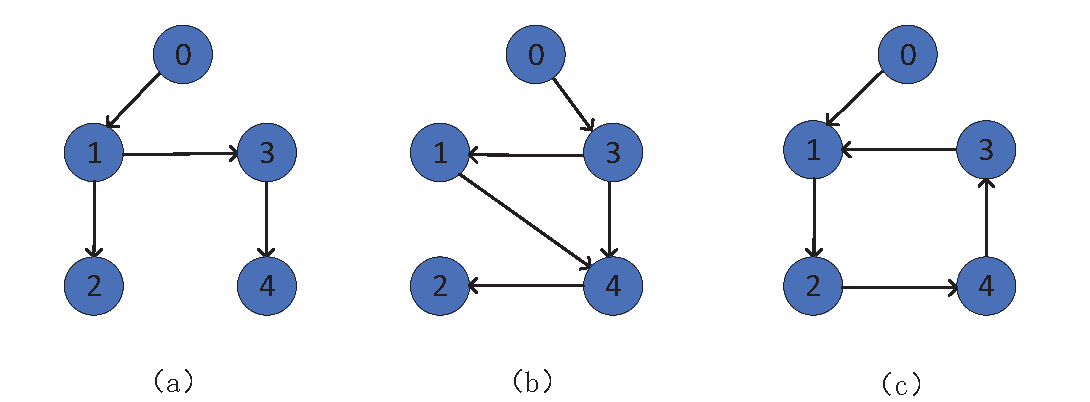
\includegraphics[scale=0.8]{./ch4/fig4-8.pdf}
    \caption{ 非线性时滞多智能体系统 (\ref{4-3-1}) 的切换拓扑   }
    \label{f4-8}
\end{figure}   
\begin{figure}[!bp]
    \centering
    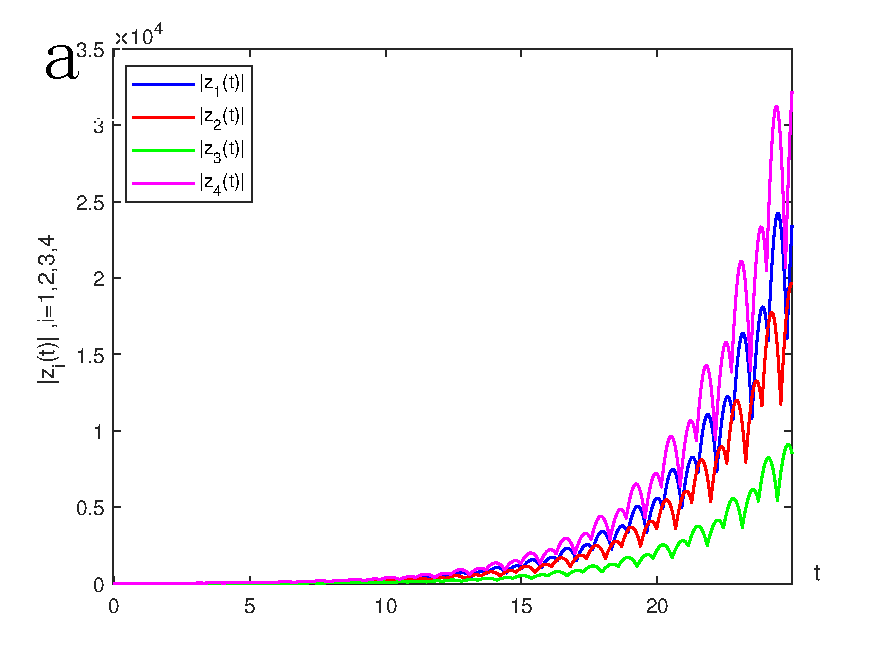
\includegraphics[scale=0.5]{./ch4/fig4-9-1.pdf}
    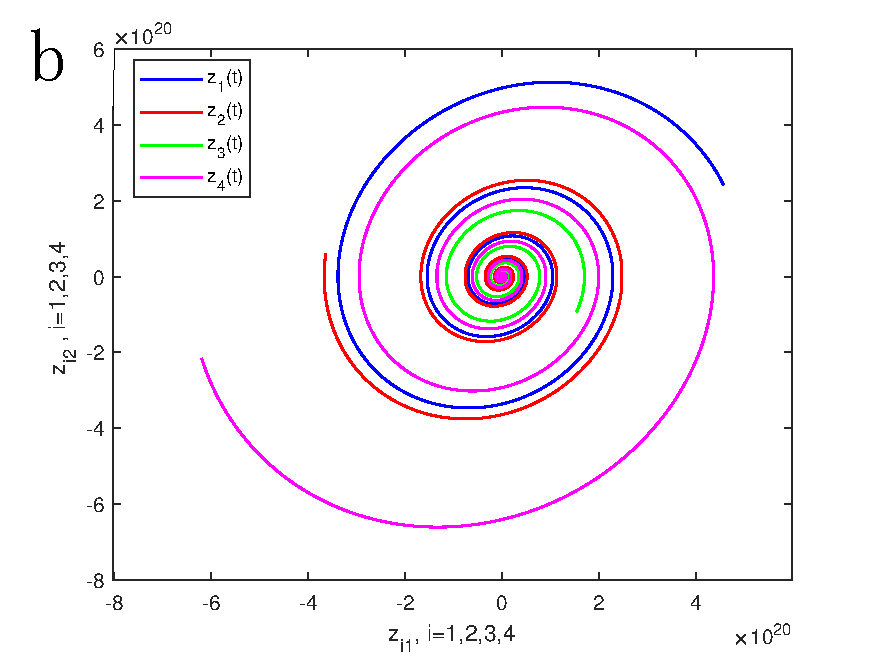
\includegraphics[scale=0.5]{./ch4/fig4-9-2.pdf}  
    \caption{无脉冲控制的误差系统 (\ref{4-3-4}) 的状态轨迹 }
    \label{f4-9}
\end{figure}

另一方面,取 $\vartheta_0=0.01$,$ 
\vartheta_1=0.03$,$\eta_1=0.89$,$
\eta_2=0.56$,$\mu_{1000}=0.9$,$
\mu_{1001}=1.11$,$  
\mu_{1010}=1.25$,$
\mu_{1011}=1.32$,$ 
\mu_{1100}=1.52$,$ 
\mu_{1101}=1.46$,$ 
\mu_{1110}=1.76$,$ 
\mu_{1111}=1.89$,$ 
\mu_{20}=0.35$,$ 
\mu_{21}=0.45$,$\gamma=0.5$,$
q=1.1$,$ 
p=2.8$,$\varepsilon_1=5/4$ 和 $
\varepsilon_2=3/2$。 因为 $\frac{\ln q}{p}=0.034> \vartheta_1=0.03$,所以条件 (\ref{4-3-10}) 是成立的。选取形状参考 $\mathscr{X}_R=\{\chi_1\}$,其中 $\chi_1=[0,1,0,1,0,1,0,1]^T$, 利用 Yalmip 求解优化问题 \textbf{Pr1},得到
\begin{align*} 
\delta^{\text{定理}\ref{t4-3-1}}_{\max}&=0.2565\\
P^{\text{定理}\ref{t4-3-1}}_0 &=\left[ \begin{array}{cc}
1.8754&0\vspace{0.2cm}\\
0&1.8754
\end{array}
\right],~~
P^{\text{定理}\ref{t4-3-1}}_1=\left[ \begin{array}{cc}
1.8899&0.0002\vspace{0.2cm}\\
0.0002& 1.8901
\end{array}\right],\\
P^{\text{定理}\ref{t4-3-1}}_2&=\left[ \begin{array}{cc}
2.2067& 0.0011\vspace{0.2cm}\\
0.0011& 2.2009
\end{array}\right],~~
F^{\text{定理}\ref{t4-3-1}} =\left[ \begin{array}{cc}
0.3060& 0.0001\vspace{0.2cm}\\
0.0001&0.3049
\end{array}\right],\\
H^{\text{定理}\ref{t4-3-1}}&=\left[ \begin{array}{cc}
0.2779& 0.0001\vspace{0.2cm}\\
0   &  0\vspace{0.2cm}\\
0.2779 &   0.0001\vspace{0.2cm}\\
0.0001 &   0.2915
\end{array}\right].
\end{align*}
因此,在具有脉冲序列 $\mathscr{F}_{[0.01,0.03]}$ 的分布式饱和脉冲控制 (\ref{4-3-2}) 下,初值满足 $\phi\in\mathscr{E}( P(t),1)$ 的非线性时滞多智能体系统 (\ref{4-3-1}) 可以实现局部领导者--跟随一致性,即误差系统 (\ref{4-3-4}) 是局部指数稳定的,如图 \ref{f4-10} 所示。 并且, 水平集  $\mathscr{E}( P(t),1)$ 是所要估计的吸引域。不同于经典的收缩不变集方法,误差系统 (\ref{4-3-4}) 的从集合 $\mathscr{E}( P(t),1)$ 内出发的状态轨迹 可以暂时离开集合 $\mathscr{E}( P(t) ,1)$ 但永远不会离开集合 $\mathscr{E}( P(t),1.1)$,也就是说集合  $\mathscr{E}( P(t) ,1)$ 将不再是不变集。 在其他条件相同的情况下,如果初值 $\phi\in\mathscr{E}( P(t),1.1)\backslash\mathscr{E}( P(t),1)$, 非线性时滞多智能体系统 (\ref{4-3-1}) 在具有脉冲序列 $\mathscr{F}_{[0.01,0.03]}$ 的分布式饱和脉冲控制 (\ref{4-3-2}) 下无法实现局部领导者--跟随一致性,即误差系统 (\ref{4-3-4}) 是不稳定的,如图 \ref{f4-11} 所示,这意味着集合 $\mathscr{E}( P(t),1.1)$ 也不是不变集。

\begin{figure}[H]
    \centering
    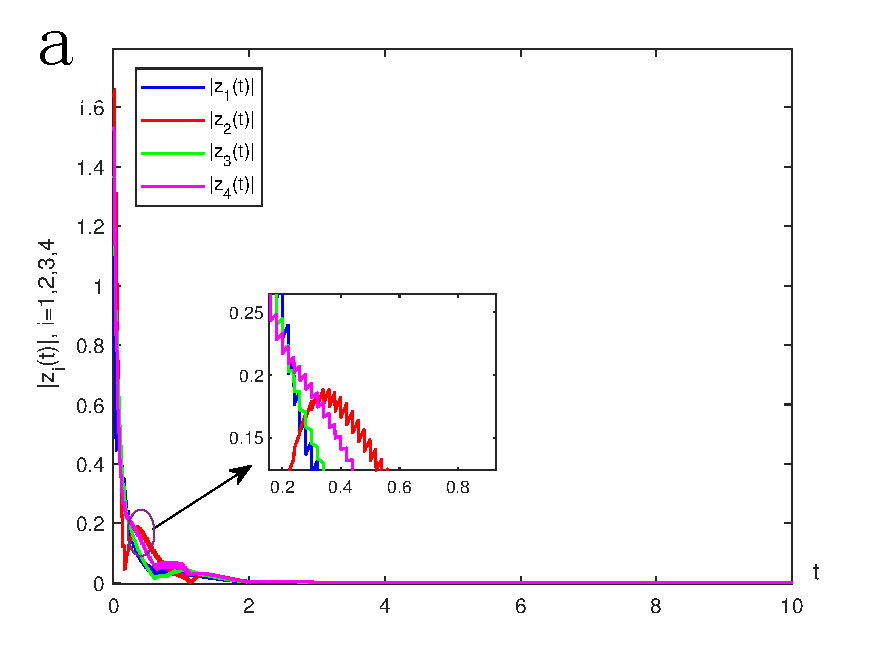
\includegraphics[scale=0.5]{./ch4/fig4-10-1.pdf}
    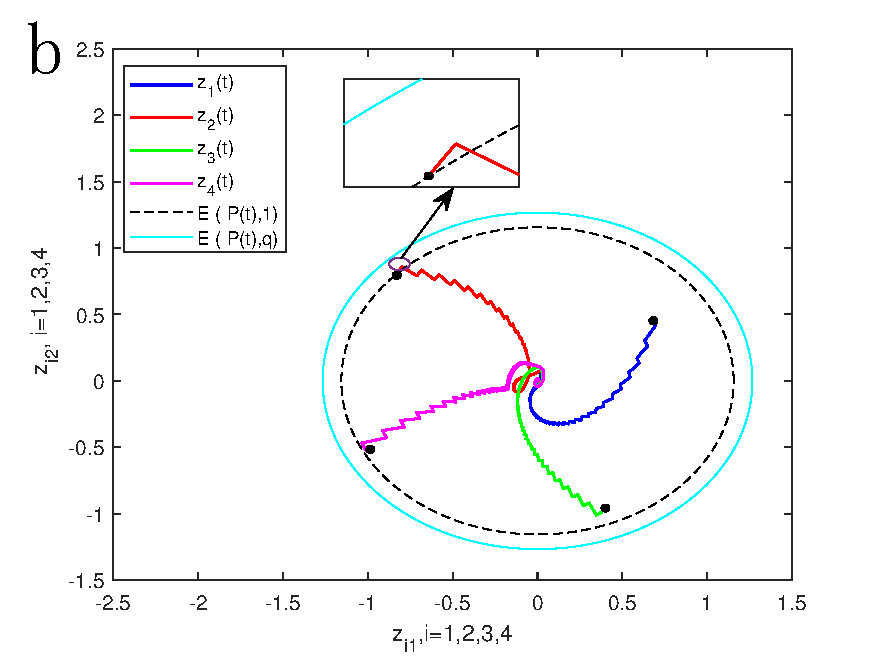
\includegraphics[scale=0.5]{./ch4/fig4-10-2.pdf} 
    \caption{具有脉冲序列 $\mathscr{F}_{[0.01,0.03]}$ 的分布式饱和脉冲控制 (\ref{4-3-2}) 下始于集合 $\phi\in \mathscr{E}( P(t),1)$ 的误差系统 (\ref{4-3-4}) 的状态轨迹}
    \label{f4-10}
\end{figure} 
\begin{figure}[H]
    \centering
    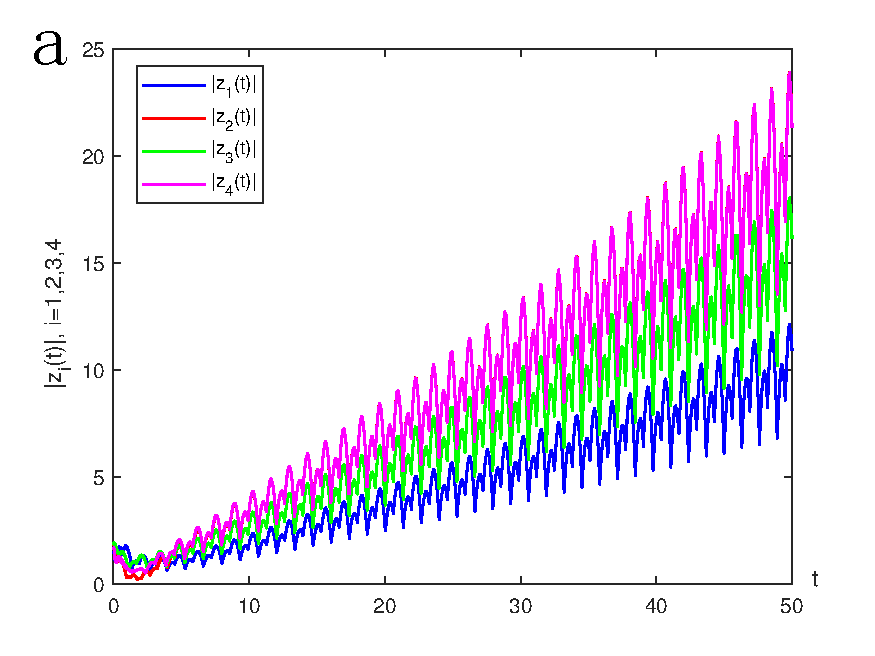
\includegraphics[scale=0.5  ]{./ch4/fig4-11-1.pdf}
    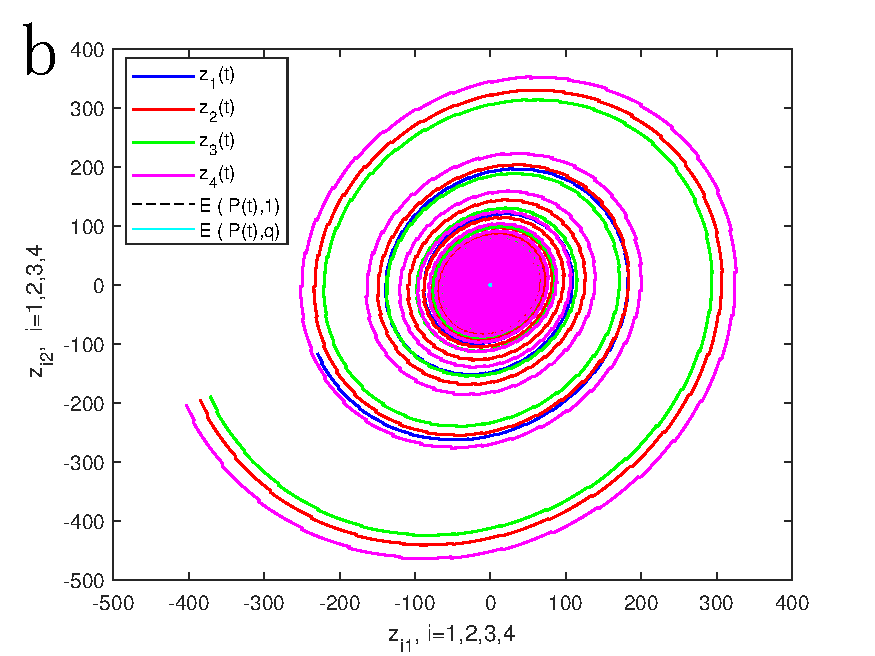
\includegraphics[scale=0.5 ]{./ch4/fig4-11-2.pdf} 
    \caption{具有脉冲序列 $\mathscr{F}_{[0.01,0.03]}$ 的分布式饱和脉冲控制 (\ref{4-3-2}) 下始于集合 $\phi\in \mathscr{E}( P(t),1.1) \backslash\mathscr{E}( P(t),1)$ 的误差系统 (\ref{4-3-4}) 的状态轨迹 }
    \label{f4-11}
\end{figure}  
\begin{figure}[H]
    \centering
    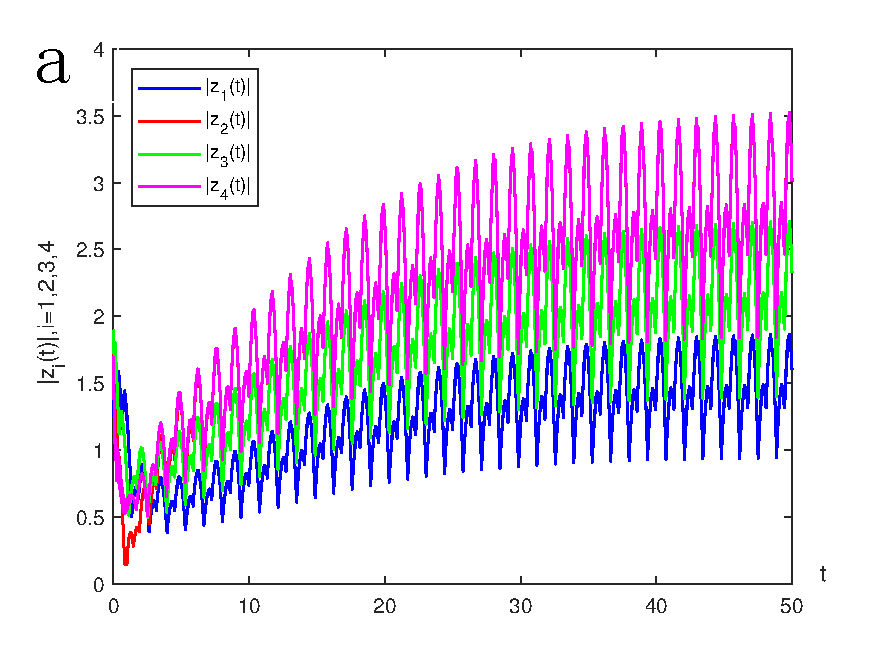
\includegraphics[scale=0.5]{./ch4/fig4-12-1.pdf}
    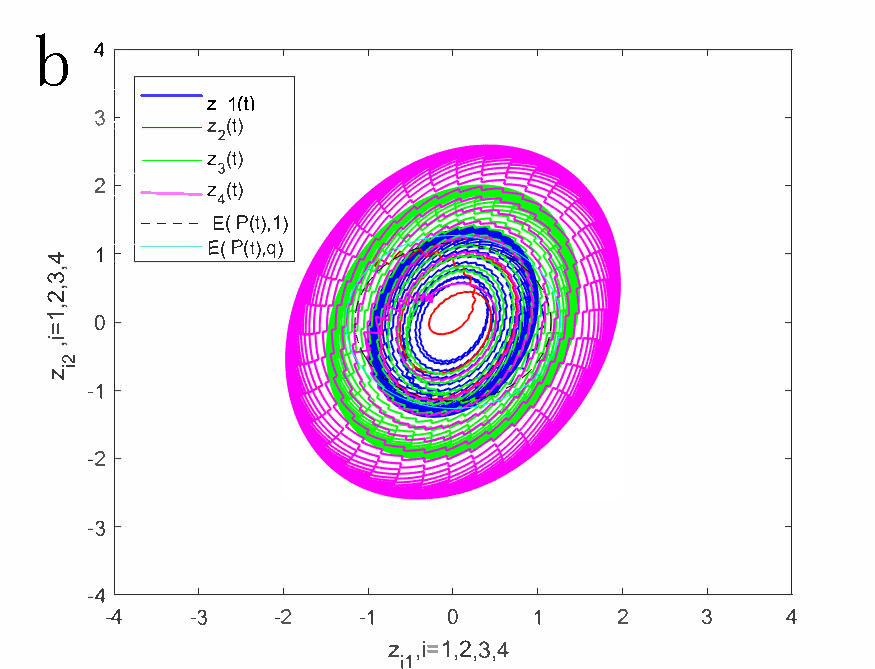
\includegraphics[scale=0.5]{./ch4/fig4-12-2.pdf} 
    \caption{具有脉冲序列 $\mathscr{F}_{[0.06,0.07]}$ 的分布式饱和脉冲控制 (\ref{4-3-2}) 下始于集合 $\phi\in \mathscr{E}( P(t),1)$ 的误差系统 (\ref{4-3-4}) 的状态轨迹}
    \label{f4-12}
\end{figure} 
另一方面,当初值 $\phi\in \mathscr{E}( P(t),1)$ 但 $\vartheta_1=0.075>\frac{\ln q}{p}=0.034$, 即定理 \ref{t4-3-1} 中的条件 (\ref{4-3-10}) 不满足,非线性时滞多智能体系统 (\ref{4-3-1}) 无法实现局部领导者--跟随一致性,即误差系统 (\ref{4-3-4}) 是不稳定的,如图 \ref{f4-12} 所示。

为了比较采用不同的饱和脉冲约束处理方法和选择不同类型的 Lyapunov 函数估计出的吸引域大小,选择相同的参数   $\eta_1=
\eta_2=1$,$\mu_{1rs\hslash}= 1$,$\mu_{2\hslash}= 0.5$,这里 $r$、$s$、$\hslash\in I[0,1]$,$q=1.04$,$
p=2.8$,$\vartheta_1=0.01$,$
\vartheta_1=0.013$, 并分别求解优化问题 \textbf{Pr1}--\textbf{4},可行解如下: 
\begin{align*} 
\delta^{Theorem \ref{t4-3-1}}_{\max}&=0.3096,\\ 
P^{Theorem \ref{t4-3-1}}_0&=\left[ \begin{array}{cc}
0.7479&  0.0000\\
0.0000&0.7478
\end{array}
\right],~
P^{Theorem \ref{t4-3-1}}_1=\left[ \begin{array}{cc}
0.7573& 0.0000\\
0.0000& 0.7573
\end{array}\right],\\  
P^{Theorem \ref{t4-3-1}}_2&=\left[ \begin{array}{cc}
0.7788 &0.0011\\
0.0011& 0.7787
\end{array}\right],\\
\delta^{Corollary \ref{c4-3-1}}_{\max}&=0.2987,\\ 
P^{Corollary \ref{c4-3-1}}_0&=\left[ \begin{array}{cc}
0.7934& 0.0000\\
0.0000& 0.7997
\end{array}
\right],~
P^{Corollary \ref{c4-3-1}}_1=\left[ \begin{array}{cc}
0.8139&0.0011\\
0.0011 &0.8109
\end{array}\right],\\ 
P^{Corollary \ref{c4-3-1}}_2&=\left[ \begin{array}{cc}
0.8491& 0.0000\\
0.0000& 0.8479
\end{array}\right],\\
\delta^{Theorem \ref{t4-3-2}}_{\max}&=0.1758,\\  
P^{Theorem \ref{t4-3-2}}&=\left[ \begin{array}{cc}
1.2049&-0.0236\\
-0.0236&0.9471
\end{array}\right],\\ \delta^{Corollary \ref{c4-3-2}}_{\max}&=0.1413,\\  
P^{Corollary \ref{c4-3-2}}&=\left[ \begin{array}{cc}
1.2610&-0.0217\\
-0.0217&1.0468
\end{array}\right]. 
\end{align*}
图 \ref{f4-13} 描绘了相应的水平集,从外往里依次对应着基于依赖于脉冲时刻的复合型 Lyapunov 函数的定理 \ref{t4-3-1}、推论 \ref{c4-3-1} 和基于二次 Lyapunov 函数的定理 \ref{t4-3-2}、推论 \ref{c4-3-2}。显然,定理 \ref{t4-3-1} 得到了最大的吸引域估计。不难发现,当选择相同类型的 Lyapunov 函数时, 采用最新的凸包表示法处理饱和脉冲项可以比传统凸包表示法 \cite{2014Global499,2017Global1270, 2018StabilityLi,2020Performance734,2013Adaptive1545,2018Event4391,2020Consensus194,2020Adaptive3013960,2019dynamic1699,li2020impulsive,shen2019estimation,HE2021126452,ouyang2020impulsive} 获得更大的吸引域估计。另一方面,无论选择哪种凸包表示法, 利用依赖于脉冲时刻的复合型 Lyapunov 函数估计出的吸引域都大于利用二次 Lyapunov 函数估计出吸引域,这表明在估计吸引域方面,依赖于脉冲时刻的复合型 Lyapunov 函数一定优于二次 Lyapunov 函数 \cite{2013Analysis871,2014Global499,2017Global1270,2020Performance734,2013Adaptive1545,2018Event4391,2020Consensus194,2020Adaptive3013960}。  
\begin{figure}[H]
    \centering
    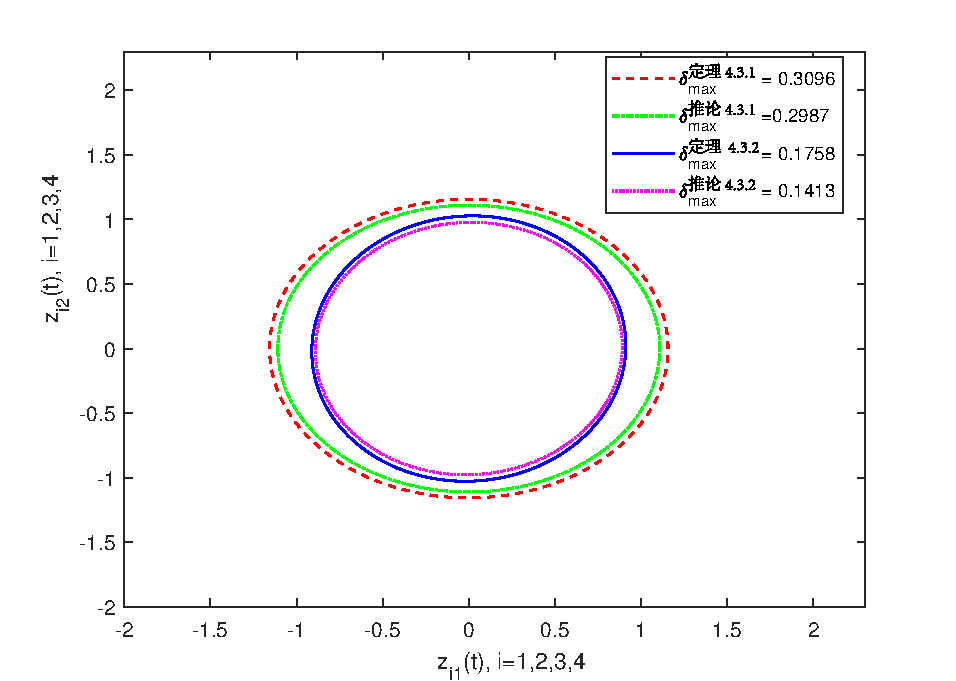
\includegraphics[scale=0.75 ]{./ch4/fig4-13.pdf}
    \caption{ 基于不同方法的吸引域估计}
    \label{f4-13}
\end{figure} 
\section{小结}

本章分析了分布式饱和脉冲控制下时滞复杂网络的局部动力学行为。首先,利用反证法、脉冲系统的比较原理和平均脉冲区间的方法研究了分布式饱和脉冲控制下具有耦合时滞的鲁里叶网络的局部指数同步问题,并给出了不依赖于时滞的基于 BMIs 的充分性判据。为了降低保守性,选取最新的具有更多松弛变量的改进凸包表示法来处理分布式饱和的脉冲项,并且开发了一种与收缩不变集完全不同的估计吸引域的方法。其次,通过构造依赖于脉冲时刻的复合型 Lyapunov 函数进一步降低保守性,讨论了分布式饱和脉冲控制下具有切换拓扑的非线性时滞多智能体系统的局部一致性,并建立了相应的局部一致性判据。为了估计出最大的吸引域,通过适当的矩阵变换,建立了基于 LMIs 的优化问题,并通过 Matlab 软件中的 Yalmip 工具箱求解相应的最大吸引域的数值解。  

本章部分结果已发表在国际期刊  IEEE Transactions on Neural Networks and Learning Systems 上,部分结果已投稿至国际期刊 IEEE
Transactions on Automatic Control。具体详见作者发表论文的清单。
